
\documentclass[acmsmall,review,anonymous]{acmart}\settopmatter{printfolios=true,printccs=false,printacmref=false}


%%
%% \BibTeX command to typeset BibTeX logo in the docs
\AtBeginDocument{%
  \providecommand\BibTeX{{%
    \normalfont B\kern-0.5em{\scshape i\kern-0.25em b}\kern-0.8em\TeX}}}
    
    \acmJournal{PACMPL}
\acmVolume{1}
\acmNumber{POPL} % CONF = POPL or ICFP or OOPSLA
\acmArticle{1}
\acmYear{2018}
\acmMonth{1}
\acmDOI{} % \acmDOI{10.1145/nnnnnnn.nnnnnnn}
\startPage{1}

\setcopyright{none}
%\setcopyright{acmcopyright}
%\setcopyright{acmlicensed}
%\setcopyright{rightsretained}
%\copyrightyear{2018}           %% If different from \acmYear




%%%%%%%%%%%%%%%%%%%%%%%%%%%%%%%%%%%%%%%%%%%%%%%%%%%%%%%%%%%%%%%%%%%%%%
%% Note: Authors migrating a paper from PACMPL format to traditional
%% SIGPLAN proceedings format must update the '\documentclass' and
%% topmatter commands above; see 'acmart-sigplanproc-template.tex'.
%%%%%%%%%%%%%%%%%%%%%%%%%%%%%%%%%%%%%%%%%%%%%%%%%%%%%%%%%%%%%%%%%%%%%%


%% Some recommended packages.
\usepackage{booktabs}   %% For formal tables:
                        %% http://ctan.org/pkg/booktabs
\usepackage{subcaption} %% For complex figures with subfigures/subcaptions
                        %% http://ctan.org/pkg/subcaption


%% Rights management information.  This information is sent to you
%% when you complete the rights form.  These commands have SAMPLE
%% values in them; it is your responsibility as an author to replace
%% the commands and values with those provided to you when you
%% complete the rights form.
\usepackage{enumerate}
\usepackage[utf8]{inputenc}
\usepackage{parcolumns}
\usepackage[spanish,english]{babel}
\usepackage{amsmath}
\usepackage{csquotes}
\usepackage{varwidth}
\newcommand{\key}[1]{\textcolor{purple}{\code{#1}}}
\newcommand{\jskey}[1]{\textcolor{blue}{\code{#1}}}
\newcommand{\es}{\textcolor{black}{\ensuremath{{es}}}}
\definecolor{palered-violet}{rgb}{0.86, 0.44, 0.58}
\definecolor{bittersweet}{rgb}{1.0, 0.44, 0.37}
\definecolor{brickred}{rgb}{0.8, 0.25, 0.33}
\definecolor{persianplum}{rgb}{0.44, 0.11, 0.11}
\newcommand{\hide}[1]{}
\newcommand{\siderule}[1]{
\code{\footnotesize{\textcolor{mGray}{#1}}}}
\usepackage{adjustbox}
\usepackage{ebproof}
\usepackage{cancel}
\newcommand{\env}{\code{\mathcal{E}}}


\usepackage{xcolor}
\definecolor{javablue}{rgb}{0.25,0,1} % for strings
\definecolor{javagreen}{rgb}{0.25,0.5,0.35} % comments
\definecolor{javapurple}{rgb}{0.5,0,0.35} % keywords
\definecolor{javadocblue}{rgb}{0.25,0.35,0.75} % javadoc
\definecolor{mGray}{rgb}{0.4,0.4,0.4}
\definecolor{mPurple}{rgb}{0.58,0,0.82}
\definecolor{huntergreen}{rgb}{0.33, 0.42, 0.18}

\definecolor{darkpastelred}{rgb}{0, 0, 0}
\definecolor{backgroundColour}{rgb}{0.95,0.95,0.92}
\definecolor{brickred}{rgb}{0.8, 0.25, 0.33}
\definecolor{red}{rgb}{0.6,0,0} 
\definecolor{blue}{rgb}{0,0,0.6}
\definecolor{green}{rgb}{0,0.8,0}
\definecolor{cyan}{rgb}{0.0,0.6,0.6}
\definecolor{cloudwhite}{rgb}{0.9412, 0.9608, 0.8471} 
\definecolor{davysgrey}{rgb}{0.33, 0.33, 0.33}
\definecolor{deepfuchsia}{rgb}{0.76, 0.33, 0.76}
\definecolor{deeplilac}{rgb}{0.6, 0.33, 0.73}
\definecolor{deepskyblue}{rgb}{0.0, 0.75, 1.0}
\definecolor{indianred}{rgb}{0.8, 0.36, 0.36}
\definecolor{airforceblue}{rgb}{0.36, 0.54, 0.66}
\definecolor{darkred}{rgb}{0.55, 0.0, 0.0}
\usepackage{wrapfig}
\newcommand{\effect}{\textcolor{black}{\ensuremath{\mathrm{\Phi}}}}
\definecolor{color_pure}{RGB}{3,35,14}
\newcommand\pure[1]{ \textcolor{black}{#1}}
\usepackage{epigraph}
\newcommand{\anyevent}[1]{{\textcolor{darkred}
{\underline{\textbf{\footnotesize #1}}}}}
\newcommand{\seq}{\cdot}
\newcommand{\choice}{\vee}
\newcommand{\fullname}{Integrated Dependent Effects}
\newcommand{\name}{integrated effects}
\newcommand{\code}[1]{{\tt{\ensuremath{\m{#1}}}}}
\newcommand{\codeme}[1]{{\tt{\ensuremath{#1}}}}
\newcommand{\esn}[2]{\ensuremath{#1^{#2}}}
\newcommand{\empt}{\textcolor{black}{\ensuremath{\epsilon}}}
\newcommand{\bott}{\textcolor{black}{\ensuremath{\bot}}}
\newcommand{\CONTAIN}{\sqsubseteq}
\newcommand{\underscore}{\textcolor{vividauburn}{\code{\_}}}
\newcommand{\m}{\mathit}  
\newcommand{\toolName}{Tvide}
\def\defeq{\ensuremath{\,\triangleq}}
\definecolor{regalia}{rgb}{0.32, 0.18, 0.5}
\newcommand{\inclusion}{\code{\mathcal{I}}}
\definecolor{mypink}{RGB}{219, 48, 122}
\definecolor{darklavender}{rgb}{0.45, 0.31, 0.59}
\definecolor{deepcerise}{rgb}{0.85, 0.2, 0.53}
\newcommand\figref[1]{Fig. \textcolor{black}{\ref{#1}}.}
\newcommand\tabref[1]{Table \textcolor{black}{\ref{#1}}.}
\newcommand\secref[1]{Sec. \textcolor{black}{\ref{#1}}}

\newcommand\theoref[1]{Theorem~\textcolor{blue}{\ref{#1}}}
\newcommand\lemmaref[1]{Lemma~\textcolor{blue}{\ref{#1}}}
\newcommand\appref[1]{Appendix~\textcolor{blue}{\ref{#1}}}
\newcommand\defref[1]{Definition~\textcolor{blue}{\ref{#1}}}
\newcommand\algoref[1]{Algorithm~\textcolor{blue}{\ref{#1}}}
\usepackage{listings}  

\lstdefinelanguage{JavaScript}{
  keywords={typeof, const, new, true, false, catch, function, return, null, catch, switch, var,async, await, if, setTimeout, this, then, while, post, else, case, break, return},
  keywordstyle=\color{blue}\bfseries,
  ndkeywords={class, export, boolean, throw, implements, import, this},
  ndkeywordstyle=\color{darkgray}\bfseries,
  identifierstyle=\color{black},
  sensitive=false,
  comment=[l]{//},
  morecomment=[s]{/*}{*/},
  commentstyle=\color{darklavender}\ttfamily,
  stringstyle=\color{red}\ttfamily,
  morestring=[b]',
  morestring=[b]"
}

\lstset{
   language=JavaScript,
   %%backgroundcolor=\color{lightgray},
   extendedchars=true,
   basicstyle=\footnotesize\ttfamily,
   showstringspaces=false,
   showspaces=false,
%frame=single
numbers=left,   
xleftmargin=1.5em, 
    numberstyle=\tiny\color{mGray},
   numbersep=10pt,
   tabsize=4,
   breaklines=true,
   showtabs=false,
   captionpos=b,
   keywordstyle=[2]\color{purple}\bfseries, %
   morekeywords=[2]{do, hiphop,every, loop,suspend, when, signal, end, present, nothing, emit,in, out, yield, module,abort, fork, par, run},
}


%\lstset{
%  frame=none,
%  xleftmargin=2pt,
%  stepnumber=1,
%  numbers=left,
%  numbersep=5pt,
%  numberstyle=\ttfamily\tiny\color[gray]{0.3},
%  belowcaptionskip=\bigskipamount,
%  captionpos=b,
%  escapeinside={*'}{'*},
%  language=JavaScript,
%  tabsize=2,
%  emphstyle={\bf},
%  stringstyle=\mdseries\rmfamily,
%  showspaces=false,
%  keywordstyle=\bfseries\rmfamily\color{deepcerise},
%  columns=flexible,
%  basicstyle=\small\sffamily,
%  showstringspaces=false,
%  morecomment=[l]\%,
%  keywordstyle=[2]\color{darklavender}, %
%  keywords={},
%    morekeywords=[2]{hiphop,emit, abour,async,Cmd,MorePlease,Sub,Success,Failure, Roll, Html, Random, NewFace, Int, String},
%  commentstyle=\color{black}\it %mypink
%}

%%
%% Submission ID.
%% Use this when submitting an article to a sponsored event. You'll
%% receive a unique submission ID from the organizers
%% of the event, and this ID should be used as the parameter to this command.
%%\acmSubmissionID{123-A56-BU3}

%%
%% The majority of ACM publications use numbered citations and
%% references.  The command \citestyle{authoryear} switches to the
%% "author year" style.
%%
%% If you are preparing content for an event
%% sponsored by ACM SIGGRAPH, you must use the "author year" style of
%% citations and references.
%% Uncommenting
%% the next command will enable that style.
%%\citestyle{acmauthoryear}
\citestyle{acmauthoryear}   %% For author/year citations

%%
%% end of the preamble, start of the body of the document source.
\begin{document}

%%
%% The "title" command has an optional parameter,
%% allowing the author to define a "short title" to be used in page headers.
\title{Automated Timed Temporal Verification
% for a Mixed Sync-Async Concurrency Paradigm
}


%% Automated Temporal Verification for Mixed Sync-Async Reactive Paradigm


%%
%% The "author" command and its associated commands are used to define
%% the authors and their affiliations.
%% Of note is the shared affiliation of the first two authors, and the
%% "authornote" and "authornotemark" commands
%% used to denote shared contribution to the research.

\author{(Anonymous Authors)}
%\author{Valerie B\'eranger}
%\affiliation{%
%  \institution{Inria Paris-Rocquencourt}
%  \city{Rocquencourt}
%  \country{France}
%}





%%
%% By default, the full list of authors will be used in the page
%% headers. Often, this list is too long, and will overlap
%% other information printed in the page headers. This command allows
%% the author to define a more concise list
%% of authors' names for this purpose.
%\renewcommand{\shortauthors}{Trovato and Tobin, et al.}

%%
%% The abstract is a short summary of the work to be presented in the
%% article.
\begin{abstract} 
To make reactive programming more concise and flexible, it is promising to deploy a mixed concurrency paradigm \cite{berry2020hiphop} that
integrates Esterel's synchrony and preemption \cite{berry1999constructive}  
with JavaScript's asynchrony \cite{madsen2017model}. 
%HipHop.js \cite{berry2020hiphop} is the first web language that 
Existing temporal verification techniques have not been designed to handle such a blending of two concurrency
models.
We propose a novel solution via a 
compositional 
Hoare-style forward verifier and a term rewriting system (TRS) on \emph{Timed Synchronous Effects} (TSE).  

Firstly, we introduce TSE, a new effects logic, that extends \emph{Kleene Algebra} with value-dependent constraints, providing real-time bounds for logical-time synchronous traces \cite{von2017real}. 
Secondly, we establish an axiomatic semantics  for a core language \code{\lambda_{HH}}, generalising the mixed paradigm. 
% HipHop.js,  based on our effects logic. 
%Secondly, we formalise a set of construction rules to infer the program effects based on a . using a set of inductive rules
Thirdly, we present a purely algebraic TRS, to efficiently check language inclusions between expressive timed effects.  
To demonstrate the feasibility of our proposals, we prototype the  verification system; prove its correctness; investigate how it can help to debug errors related to both synchronous and asynchronous programs. 


\end{abstract}

%%
%% The code below is generated by the tool at http://dl.acm.org/ccs.cfm.
%% Please copy and paste the code instead of the example below.
%%


\ccsdesc[500]{Theory of computation~Logic}
\ccsdesc[300]{Theory of computation~Semantics and reasoning}
\ccsdesc[100]{Models of computation~Concurrency}

  
  

%%
%% Keywords. The author(s) should pick words that accurately describe
%% the work being presented. Separate the keywords with commas.
\keywords{Temporal Verification,
Dependant Effects,
Hoare-style Forward Verifier,
Term Rewriting System,
Reactive System Design}


%%
%% This command processes the author and affiliation and title
%% information and builds the first part of the formatted document.
\maketitle

\section{Introduction}
\label{Introduction}

As it recently proposed,  reactive languages such as Hiphop.js\footnote{Hiphop.js is a JavaScript extension of Esterel \cite{berry1992esterel}
(or vice versa)
for reactive web applications: \url{https://www-sop.inria.fr/members/Colin.Vidal/hiphop/}.}   \cite{vidal2018hiphop,berry2020hiphop} are designed to be
based on a smooth integration of (i) Asynchronous concurrent programs, which perform interactions between components or with the environment with uncontrollable timing, such as network-based communication; (ii) Synchronous reactive programs, which react to external events in a conceptually instantaneous and deterministic way; and (iii) Preemption, the explicit cancellation and resumption of an ongoing orchestration subactivity. 


%Recent research has 

%One of the major difficulties of reactive web programming is \emph{callback hell} \cite{kambona2013evaluation}, which is the problem of appropriately handling the asynchronous events appearing in program executions. To avoid using callbacks, efforts have been made: 
%%\cite{madsen2017model}
%(i) JavaScript has provided  \emph{promises} and \emph{async/await} primitives, making it possible to chain asynchronous actions in a specific sequential order; (ii) High-level abstractions such as \emph{Functional Reactive Programming} has been carried up to the web applications \cite{czaplicki2013asynchronous}, which adopts the data flow declarative programming style: when a variable is modified, any expression that references it is implicitly reevaluated. 
%
%To go further with this problem and achieve a better web orchestration,  the language Hiphop.js \cite{vidal2018hiphop,berry2020hiphop} is designed to be a JavaScript extension of Esterel \cite{berry1992esterel} (or vice versa) based on a smooth integration of (i) Asynchronous concurrent programs, which perform interactions between components or with the environment with uncontrollable timing, such as network-based communication; (ii) Synchronous reactive programs, which react to external events in a conceptually instantaneous and deterministic way; and (iii) Preemption, the explicit cancellation and resumption of an ongoing orchestration subactivity. 




\textit{"Such a combination makes reactive programming more powerful and flexible than plain JavaScript because it makes the temporal geometry of complex executions explicit instead of hidden in implicit relations between state variables." \cite{berry2020hiphop}}

Given such a multi-paradigm (mixed Sync-Async) concurrency model, the verification of its temporal behaviour becomes engaging and challenging. 
%which, however, has not been intensely exploited. 
Existing techniques are based on a transformation to convert the asynchronous chunk into semantically equivalent synchronization\footnote{Usually the transformation is incomplete, i.e., not all the asynchronous programs can be translated into a semantically equivalent synchronization.}; then reason about the behaviours based on the synchronous semantics \cite{damian2019communication,gleissenthall2019pretend,tarawneh2018formal}. This approach (i) suffers from the limited expressiveness, restricted by finite-state automata (FSA); (ii) lacks the modularity to reason about programs compositionally; (iii) loses time awareness due to the conversion to synchronous models; and (iv) has the \emph{state explosion problem}  when proving language inclusions between FSA.
 %finite-state automata
 % PSPACE-complete complexity 

To tackle the above issues and exploit the best of both synchronous and asynchronous concurrency models, we propose a novel temporal specification language, which enables a compositional verification via a  Hoare-style forward verifier and a term rewriting system (TRS). 
More specifically, we specify system behaviours in the form of \emph{Timed Synchronous Effects (TSE)}, which integrates the Synchronous Kleene Algebra (SKA) \cite{prisacariu2010synchronous,broda2015deciding} with dependent values and arithmetic constraints, 
%gaining the expressive power beyond finite-state machines; and (ii) introduces a new parallel operator 
to 
%capture the parallelism between event-triggered (sync) and  time-triggered (async) execution traces, 
provide real-time abstractions into traditional synchronous verification. 
%Resource usages, provided by a \emph{dynamic ticks}\cite{von2017real}, incorporating the time-triggered (physical time) and event-triggered (logical time) execution loops. 
For example, one safety property, \textit{"The event \anyevent{Done} will be triggered no later than one second"}\footnote{For simplicity, we  follow the convention of JavaScript, and use integer values to represent milliseconds in this paper, while it can be easily extended to real numbers and other time measurement units.}, is expressed in our effects logic as: 
\begin{align*}
&\code{\effect \defeq \  0 {\leq} t {<}1000 : (\{{\anyevent{}\}^\star} \cdot \{\anyevent{Done}\} ) \# t}.
\end{align*}  
%The timed effects incorporates different kinds of existing temporal logics, such as linear-time temporal logic (LTL)
%and .
%which replaces temporal operators by time-constrained versions from 
Here, \code{\#} is the parallel operator specifying the \emph{real-time} constraints for the \emph{logical-time} sequences \cite{von2017real}; 
curly braces \code{\{\}} enclose a single  logical-time instance\footnote{A time instance is a set of signals (possible empty) with status, logically concurring at the same time (cf. {\secref{subsec:Specification_language}}).}; 
Kleene star \code{\star} denotes trace repetition.
The above formula \code{\effect} corresponds to `\code{\Diamond_{[0, 1000)}\ }\anyevent{Done}' in metric temporal logic (MTL), reads \textit{"within one second, \anyevent{Done} finally happens"}. Moreover, the time bounds can be dependent on the program inputs. For example, we express, the effects of \code{send(d)} as:
\begin{align*}
&\code{\effect^{send (d)} \defeq \  (0 {<} d {\leq}5000 \wedge  0 {\leq} t {<} d) : (\{{\anyevent{Send}\} \# t)} \cdot \{\anyevent{Done}\}}.
\end{align*}  
The \code{send} method takes a parameter \code{d}, and \anyevent{Send}s out a message at time \code{t}.  
The above formula  \code{\effect^{send (d)}} indicates that the input  \code{d} is positive and smaller or equal to \code{5000}; the method generates a finite trace, with the first time instance containing the event \anyevent{Send}, followed by a second time instance containing the event \anyevent{Done}; and the instance \code{\{}\anyevent{Send}\code{\}} takes a no more than \code{d} milliseconds delay to finish. 
Although these examples are simple, they show the benefits of deploying value-dependent time bounds. Intuitively, if traditional timed automata \cite{larsen1997uppaal} define an \emph{exact} transition system, our timed effects define a set (possibly infinite) of exact transition systems. 



 
   
   %they already illustrate the gain of expressiveness from  existing temporal logics and traditional timed automata. 

%properties beyond 





Having the effects logic as the specification language, we are interested in the following verification problem: 
Given a program \code{\mathcal{P}}, and a temporal property \code{\effect^{\prime}}, does \code{\effect^{\mathcal{P}} \CONTAIN \effect^{\prime}} holds? In a typical verification
context, checking the inclusion/entailment between the program effects \code{\effect^{\mathcal{P}}} and the valid traces \code{\effect^{\prime}} proves that: the program \code{\mathcal{P}} will never lead to unsafe traces which violate \code{\effect^{\prime}}.


Traditional ways of temporal verification either (i) rely on a translation from specification languages, such as LTL or CSP, into finite state automata \cite{sun2009pat}, which potentially gives rise to an exponential blow-up; %such as NFAs or DFAs; 
or (ii) use expressive automata to model the program logic directly, such as timed automata, which fails to capture the bugs introduced by the real implementation. 

In this paper, we present a new solution of extensive temporal verification comprising: a front-end verifier computes the program's  temporal behaviour, to be the \code{\effect^{\mathcal{P}}}, via inference rules at the source level; %defining program evaluation syntactically; 
and a back-end TRS, to soundly check \code{\effect^{\mathcal{P}} \CONTAIN \effect^{\prime}}. 




The TRS  is inspired by Antimirov and Mosses’ algorithm \cite{antimirov1995rewriting}\footnote{Antimirov and Mosses' algorithm was designed for deciding the inequalities of regular expressions based on an 
complete 
axiomatic algorithm of the algebra of regular sets.} but solving the language inclusions between more expressive timed synchronous effects.  A TRS is a refutation method that normalizes expressions in such a way that checking their inclusion corresponds to an iterated process of checking the inclusion of their \emph{partial derivatives} \cite{antimirov1995partial}. 
Works based on such a TRS \cite{song2020automated,antimirov1995rewriting,almeida2009antimirov,keil2014symbolic,hovland2012inclusion}  show its feasibility and suggest that this method is a better average-case algorithm than those based on the comparison of automata. 


This work targets timed temporal verification, and to the best of the authors’ knowledge, it proposes the first axiomatic semantics and the first algebraic TRS (proven sound and complete) for the mixed synchronous and asynchronous concurrency model.  Our main contributions are:% as follows:



\begin{enumerate}
\item \textbf{The Timed Synchronous Effects:} We define the syntax ({\secref{subsec:Specification_language}}) and semantics ({\secref{subsec:Specification_Semantics}}) of timed synchronous effects, to be the specification language, which captures the target programs' behaviours and non-trivial temporal properties.

\item \textbf{Automated Forward Verifier:} Targeting a core language \code{\lambda_{HH}} ({\secref{subsec:Targetlanguage}}), we 
establish its axiomatic semantics via a set of inductive transition rules (\secref{sec:Verification}), enabling a compositional verifier to infer the program's effects. The verifier triggers the back-end solver TRS. 

%which tightly The semantics model closely captures the temporal behaviour of the program, 

\item \textbf{An Efficient TRS:}
We present the rewriting rules, to prove 
the inferred effects against given temporal properties, both expressed by timed synchronous effects (\secref{sec:Entailment_Prover}). 


\item \textbf{Implementation and Evaluation:} We prototype the novel effects logic and the automated verification system, %on top of the HIP/SLEEK system\cite{chin2012automated}, 
%which is available online\cite{Demo}, 
prove the correctness, report on a case study investigating how it can help to debug errors related to both synchronous and asynchronous programs (\secref{subsec:Case_Studies}).


\end{enumerate} 



\noindent\textbf{\textit{Organization.}} 
\secref{sec:Preliminaries} introduces the language features of synchronous Esterel programs, JavaScript promises, and the web reactive language HipHop.js. 
\secref{sec:Overview} gives motivation examples to highlight the key methodologies and contributions. 
\secref{sec:LanguageSpecifications} formally presents the core   language \code{\lambda_{HH}}, and the syntax and semantics of timed synchronous effects.
\secref{sec:Verification} presents the forward verification rules.
\secref{sec:Entailment_Prover} explains the TRS for effects inclusion checking, and displays the essential auxiliary functions. 
\secref{sec:Evaluation} demonstrates the implementation and cases studies. % via a number of . 
We discuss related works in \secref{sec:Related_work} and conclude in  \secref{sec:conclusion}. Omitted proofs can be found in the Appendix.


\section{Background: Esterel, Async-Await, and Hiphop.js }
\label{sec:Preliminaries}

It has been an active research topic to build flexible programming paradigms for reactive systems in different domains. This section identifies: i) \emph{Synchronous programming}, represented by Esterel  \cite{berry1992esterel}, ii) \emph{Asynchronous programming}, represented by JavaScript promises \cite{madsen2017model}, and iii) A \emph{mixed Sync-Async} paradigm, recently proposed by HipHop.js  \cite{berry2020hiphop}. Meanwhile, we discuss the real-world programming challenges of each paradigm; and show how our proposal addresses them in the cases studies, \secref{subsec:Case_Studies}. 

 
 




 %language abstractions 

\subsection{A Sense of Esterel: Synchronous and Preemptive}

%Synchronous programming (also synchronous reactive programming or SRP) is a computer programming paradigm supported by synchronous programming languages. 

The principle of synchronous programming is to design a high-level abstraction where the timing characteristics of the electronic transistors are neglected \cite{esterel_wiki}. Such an abstraction makes reasoning about time a lot simpler, thanks to the notion of \emph{logical ticks}: a synchronous program reacts to its environment in a sequence of ticks, and computations within a tick are assumed to be instantaneous. 
As one of the first few well-known synchronous languages, Esterel's high-level imperative style allows the simple expression of parallelism and preemption, making it natural for programmers to specify and reason about control-dominated model designs. Esterel has found success in many safety-critical applications such as nuclear power plant control software. The success with real-time and embedded systems in domains that need strong guarantees can be partially attributed to its precise semantics and computational model  \cite{berry1992esterel,berry1999constructive, song2021synchronous}. 

Esterel treats computation as a series of deterministic reactions to external signals. All parts of a reaction complete in a single, discrete-time step called an \emph{instance}. Besides, instances exhibit deterministic concurrency; each reaction may contain concurrent threads without execution order affecting the computation result. Primitive constructs execute in zero time except for the \code{yield} (pause) statement. Hence, time flows as a sequence of logical instances separated by explicit pauses. In each instance, several elementary instantaneous computations take place simultaneously. 


\begin{lstlisting}
fork {emit A; yield; emit B; emit C} par {emit E; yield; emit F; yield; emit G}
\end{lstlisting}  


The synchronous parallelism in Esterel is constructed by the \code{\m{fork} \{...\} \m{par}  \{...\}  } statement. 
It remains active as long as one of its branches remains active, 
% unless some branch exits a trap, 
and it terminates when both branches are terminated. The branches can terminate in different instances, and wait for the last one to terminate.
As the above example shows, the first branch generates effects $\{\textbf{A}\} \cdot \{\textbf{B}, \textbf{C}\}$ while the second branch generates effects $\{\textbf{E}\} \cdot \{\textbf{F}\} \cdot \{\textbf{G}\}$; then the final effects should be $\{\textbf{A},\textbf{E}\}\cdot \{\textbf{B}, \textbf{C}, \textbf{F}\} \cdot \{\textbf{G}\}$. 


To maintain determinism and synchrony, evaluation in one thread of execution may affect code arbitrarily far away in the program. In other words, there is a strong relationship between signal status and control propagation: a signal status determines which branch of a \code{present} test is executed, which in turn determines which \code{emit} statements are executed (See \secref{subsec:Targetlanguage} for the language syntax). 
%For instance, selecting a particular branch of execution in one thread may immediately unblock a different thread of execution. 
%The selection of the other branch may render the entire program invalid\citeref{florence2019calculus}. 
The first semantic challenge of programming Esterel is the \emph{Logical Correctness} issue, caused by these non-local executions, which is simply the requirement that there exists precisely \textbf{one} status for each signal. For example, consider the program below:

\begin{lstlisting}
signal S1 in present S1 then nothing else emit S1 end present end signal
\end{lstlisting}  

If the local signal {\textbf{S1}} were \emph{present}, the program would take the first branch of the condition, and the program would terminate without having emitted {\textbf{S1}} (\code{nothing} leaves \code{\textbf{S1}} with   \emph{absent}). If \code{\textbf{S1}} were absent, the program would choose the second branch and emit the signal. Both executions lead to a contradiction. Therefore there are no valid assignments of signals in this program. This program is logically incorrect.


\begin{lstlisting}
signal S1 in present S1 then emit S1 else nothing end present end signal
\end{lstlisting}  

Consider the revised program above. If the local signal {\textbf{S1}} were present, the conditional would take the first branch, and  {\textbf{S1}} would be emitted, justifying
the choice of signal value. 
If {\textbf{S1}} were absent, the signal would not be emitted, and the choice of absence is also justified. Thus there are two possible assignments to the signals in this program, which is also logically incorrect.

\begin{wrapfigure}{R}{0.41\columnwidth}
    \vspace{-1mm}
\centering
\begin{lstlisting}
module a_loop: output A,B,C;
  emit A;
  loop 
  	emit B; yield; emit C
  end loop  
end module
\end{lstlisting}  
     \vspace{-1mm}
 \caption{A Loop Example in Esterel \cite{song2021synchronous}.} 
  \label{fig:loop1}
       \vspace{-1mm}
\end{wrapfigure}

Esterel's instantaneous nature requires a special distinction when it comes to loop statements, which increases the difficulty of the effects invariants inference.  
As shown in \figref{fig:loop1}, the program firstly emits signal {\textbf{A}}, then enters into a loop which emits signal \code{\textbf{B}} followed by a \code{\m{yield}} followed by emitting signal {\textbf{C}} at the end. 
The effects of it is $ \{\textbf{A}, \textbf{B}\} \cdot \{ \textbf{B}, \textbf{C}\} \cdot \{ \textbf{B}, \textbf{C}\} \cdot \{ \textbf{B}, \textbf{C}\} ...$,
which says that in the first time instance, signals {\textbf{A}} and {\textbf{B}} will be present, 
as there is no explicit yield between $emit\ \textbf{A}$ and $emit\ \textbf{B}$; 
then for the following instances (in an infinite trace), signals {\textbf{B}} and {\textbf{C}} are present all the time, because after executing $emit\ \textbf{C}$, it immediately executes from the beginning of the loop, which is $emit\ \textbf{B}$. 


 %one deals with concurrent processes that coordinate with each other. 


Coordination in concurrent systems can result from information exchange, using messages circulating on channels with possible implied synchronization. In Esterel, it can also result from \emph{process preemption}  \cite{berry1993preemption}, which is a more implicit control mechanism that consists in denying the right to work to a process, either permanently (abortion, cf. \figref{fig:overview_eg1}) or temporarily (e.g. suspension). Preemption is particularly important in control-dominated reactive and real-time programming, where most of the works consist of handling interrupts and controlling computation.  



%
%\begin{wrapfigure}{L}{0.4\columnwidth}
%    \vspace{-1mm}
%\centering
%\begin{lstlisting}
%suspend
%	loop emit A; yield; yield;
%	end loop
%when B end suspend
%\end{lstlisting}  
%     \vspace{-1mm}
% \caption{A Suspend Example in Esterel.} 
%  \label{fig:Suspend}
%       \vspace{5mm}
%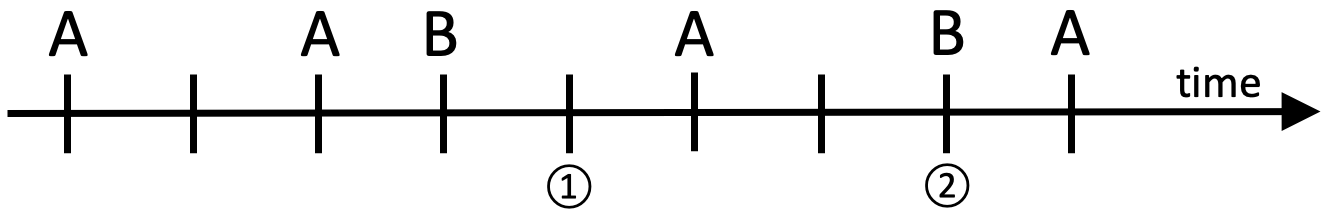
\includegraphics[width=0.39\columnwidth]{suspend.png}
%        \vspace{-1mm}
%\caption{\label{fig:Suspend}Graphical Illustration of \figref{fig:Suspend}}
%        \vspace{0mm}
%\end{wrapfigure}
%
%
%\figref{fig:Suspend} presents a suspend statement, one of the preemptive operations in Esterel. When the preemption condition satisfied, it pauses the execution of a group of statements, and resume it from the next time instance. 
%As \figref{fig:Suspend_pbg} illustrates, without the preemption, the effects is a repeated pattern: \code{\{\textbf{A}\}\cdot\{\}\cdot\{\textbf{A}\}\cdot\{\} \cdot ...} . Due to the presence of signal \code{\textbf{B}}, it delays emission of \code{\textbf{A}} by one cycle (at {\textcircled{1}} and {\textcircled{2}}), and resumes from the next cycle. 

While the flexibility they provide us, preemption primitives often with loose or complex semantics, making abstract reasoning difficult. 
Most existing languages offer a small set of preemption primitives, often insufficient to program reactive systems concisely. 







\subsection{Asynchrony from JavaScript Promises: Async–Await}

\noindent \textit{"Who can wait quietly while the mud settles? Who can remain still until the moment of action?"}\\
\textcolor{white}{.}\qquad\qquad\qquad\qquad\qquad\qquad\qquad\qquad\qquad\qquad\qquad\qquad\qquad\qquad\qquad \textit{ -- Laozi, Tao Te Ching}


A number of mainstream languages, such as C\code{\#}, JavaScript, Rust, and Swift, have recently added support for async–await and the accompanying promises abstraction\footnote{JavaScript's asynchrony arises in situations such as web-based user-interfaces, communicating with servers through HTTP requests, and non-blocking I/O.}, also known as \emph{futures} or \emph{tasks} \cite{bierman2012pause}. As an example, consider the JavaScript program in \figref{fig:json}, 
it uses the {\ttfamily{fs}} module (line 1) to load the file into a variable (line 6) using async/await syntax. 



\begin{figure}[h]
    \vspace{-2mm}
\centering
\begin{lstlisting}
const fs = require('fs').promises;

async function read (filePath) {
	const task = fs.readFile(filePath);
    ... // do things that do not depend on the result of the loading file
    const data = await task; // block execution until the file is loaded
	... // logging or data processing of the Json file 
}
\end{lstlisting}  
     \vspace{-3mm}
 \caption{Using Async-Await in JavaScript.} 
  \label{fig:json}
       \vspace{-2mm}
\end{figure}




The function {\ttfamily{read}} accepts one argument, a string called {\ttfamily{filePath}}. As it is declared {\textbf{\color{blue}\ttfamily{async}}}, reading a file (line 4) does not block computations that do not depend on the result (line 5). The programmer {\textbf{\color{blue}\ttfamily{await}}}s the task when they need the result to be ready. Reading a file may raise exceptions (e.g., the file is non-existent), then the point for such an exception to emerge is where the tasks are awaited (lines 6). While await sends a signal to a task scheduler on the runtime stack, the exceptions appear to propagate in the opposite direction, from the runtime to the await sites.

Unfortunately, existing languages that support async–await do not enforce at compile time that exceptions raised by asynchronous computations are handled. The lack of this static assurance makes asynchronous programming error-prone. For example, the JavaScript compiler accepts the program above without requiring that an exception handler to be provided, which leads to program crashes if the asynchronous computation results in an exception. 
%The worse situation is: an exception raised asynchronously is possibly silently swallowed if not otherwise caught. 
Such unhandled exceptions have been identified as a common vulnerability in JavaScript programs \cite{madsen2017model,alimadadi2018finding}.
Furthermore, \cite{madsen2017model,alimadadi2018finding} display a set of other \emph{anti-patterns} including: 
attempting to settle a promise multiple times; unsettled promises; unreachable reactions; 
%implicit returns in reactions; 
and unnecessary promises, which are mostly caused by using promises without sufficient static checking. 






   \vspace{2mm}
\subsection{HipHop.js -- A mixture of Esterel and JavaScript}
\label{subsection:HipHop}

\begin{figure}[h]
\noindent
   \vspace{-2mm}
\begin{varwidth}{.5\textwidth}
\begin{lstlisting}
function enableLoginButton(){
  return (Rname.length >= 2 
	   && Rpasswd.length >= 2);}
function nameKeypress(value){
  Rname = value;
  RenableLogin=enableLoginButton();}
function passwdKeypress(value){ 
  Rpasswd = value;
  RenableLogin=enableLoginButton();}
\end{lstlisting}
\end{varwidth}%
\begin{varwidth}{.5\textwidth}
\begin{lstlisting}
hiphop module Identity(
			in name, in passwd, 
			out enableLogin){
  do{
	  emit enableLogin(
		  		name.length >= 2 
		  	 && passwd.length >= 2); 
  } every(name || passwd)
}
\end{lstlisting}  
\end{varwidth}
      \vspace{0mm}
\caption{A comparison between JavaScript (left) and HipHop.js (right) for a same login button implementation \cite{berry2020hiphop}. (On the right, {\ttfamily{name}}, {\ttfamily{passwd}} and {\ttfamily{enableLogin}} are reactive input/output signals.)}
  \label{fig:login_compare}  
      \vspace{0mm}
\end{figure}





HipHop.js is a reactive web language that adds synchronous concurrency and preemption to JavaScript, which is compiled into plain  JavaScript and executes on runtime environments \cite{berry2020hiphop}. 
To show the advantages of such a mixture, \figref{fig:login_compare} presents a comparison between JavaScript and HipHop.js to achieve the same login button. Here, {\ttfamily{Rname}}, {\ttfamily{Rpasswd}}, {\ttfamily{RenableLogin}} are global variables to model the application's states. Dis/En-abling login is done by setting {\ttfamily{RenableLogin}}. However, while more and more features get added to the specification, state variable interactions can lead to a large number of implicit and  invisible global control states.


Whereas, HipHop.js simplifies and modularizes designs, and synchronous signaling makes it possible to instantly communicate between concurrent statements to exchange data and coordination signals. 
Second, powerful event-driven reactive preemption borrowed from Esterel finely controls the lifetime of the arbitrarily complex program statements they apply, instantly killing them when their control events occur. 
More examples are discussed in the following sections.

%Third, an extension of async that synchronously signals termination completion to concurrent statements and automatically performs automatic resource cleaning when preempted. 

%






\section{Overview}\label{sec:Overview}
%We now give a summary of our techniques using running examples. 

%\subsection{HipHop.js and Dependent Effects}
\subsection{Timed Synchronous Effects}
As shown in \figref{fig:overview_eg1}, we define Hoare-triple style specifications (enclosed in \textcolor{darklavender}{\ttfamily{{/*@ ... @*/}}}) for each program, which leads to a compositional verification strategy, where static checking and timed temporal verification can be done locally. %The set of signals to be present in one logical time instance are represented within one \code{\{\}}.

\begin{figure}[h]
      \vspace{0mm}
\begin{lstlisting}[columns=fullflexible]
hiphop module authenticate(var d, var name, var passwd, in Tick, out Connecting, out Connected)
/*@ requires d>3000 : {}^*.{Login} @*/
/*@ ensures	(3000<t/\t<d : {Connecting}#t.{Connected}) \/ (t=d :  {Connecting}#t) @*/
{
   abort count(d, Tick) { // Abort the execution at d milliseconds
      async Connected {
         emit Connecting; 
         // Execute authenticateSvc after a 3000 milliseconds' delay
         setTimeout (authenticateSvc(name, passwd).post().then( v => this.notify(v)), 3000);}}}
\end{lstlisting}  
      \vspace{0mm}
      \caption{Dependent Values for Time Bounds (the program is from  \cite{berry2020hiphop}).}\label{fig:overview_eg1}
         \vspace{0mm}
\end{figure}


The {\ttfamily{authenticate}} module checks the validity of the identity at each click on login button. The operations of requesting the server are wrapped in an {\textbf{\color{purple}\ttfamily{abort}}} statement, which preempts the execution when the responding time goes beyond \code{\m{d}} (given signal \code{\anyevent{Tick}} is present every second).


After emitting the signal \anyevent{Connecting}, it emits  \anyevent{Connected} if the connection succeeds before the  preemptive deadline; otherwise, no signal is emitted. 
The precondition \code{d{>}3000 : \{
\}^\star \cdot\{\m{Login}\} } requires that the input variable \code{d} is greater than 3000, and before entering into this module, the signal \anyevent{Login} should be emitted at the last time instance, indicating that a login request has been sent. 
The postcondition contains two parts and connected using the disjunction mark \code{{\vee}}: when \code{3000{<}t{<}d}, the effects contains two time instances, \code{\{\m{Connecting}\}} and \code{\{\m{Connected}\}}, while the first  time instance finishes at time \code{t}, %(assuming to reset the clock when executing the module), 
which is no later than \code{\m{d}} milliseconds; otherwise, the effects contains one time instance \code{\{Connecting\}} which finishes at time \code{d}. \emph{(See a demo from \cite{CODE1})}



As for another example, shown in \figref{fig:overview_eg2}, the module {\ttfamily{main}} %contains a \code{\m{fork/par}   } statement, which 
spawns two threads running in  parallel.
The first thread firstly waits for the signal \anyevent{Ready}, then emits  \anyevent{Go}. 
The second thread firstly emits  \anyevent{Prep}, then calls the function {\ttfamily{cook}} asynchronously. 
The precondition of {\ttfamily{main}} requires no arithmetic constraints on its input values (expressed as \code{\m{true}}), neither any pre-traces  (expressed as \code{\m{emp}} or \code{\epsilon}, indicating an empty trace). The postcondition ensures a trace, where the second time instance contains at least one signal \code{\anyevent{Cook}} and finishes within 3000 milliseconds after the completion of the first time instance. Then we do not care about the rest of the trace (\code{\{\}} is similar to a wildcard). 
%We omit the implementation of \code{cook} here, while provide the specifications of it. 
Taking {\ttfamily{main}} as an example, the work flow of the forward verifier is presented in the following sub-section. \emph{(See a demo from \cite{CODE2})}

\begin{figure}[h]
      \vspace{-2mm}
\begin{lstlisting}[columns=fullflexible]
hiphop module main (out Prep, in Tick, out Ready, out Go, out Cook)
/*@ requires true : emp @*/
/*@ ensures  0<=t/\t<3000 : {}.({Cook})#t.{}^* @*/
{
	fork{ // The effects of the first thread is true : Ready?.{Go}
		await Ready; emit Go; 
	}par{ // The effects of the second thread is 0<t<3000 : {Prep, Cook}#t.{Ready}
		emit Prep;
		async Ready { run cook (3000, Tick, Cook); }}}
// The final effects for main is  0<=t/\t<3000 : ({Prep}.{Cook})#t.{Ready}.{Go} 
      
hiphop module cook (var d, in Tick, out Cook)
/*@ requires d>2000  : {}^*.{Prep} @*/
/*@ ensures  0<=t/\t<d : ({}.{Cook})#t @*/
{	abort count(d, Tick) { yield; emit Cook; }}
\end{lstlisting}  
      \vspace{-1mm}
      \caption{Mixed Synchronous and Asynchronous Concurrency with Function Calls.}\label{fig:overview_eg2}
            \vspace{-1mm}
\end{figure}

%We demonstrate  

%%, and a function call from module \code{main} to \code{cook}.

      \vspace{-2mm}
\subsection{Forward Verification}
As shown in \figref{fig:forward_example}, we demonstrate the forward verification process of the module  {\ttfamily{main}}. The program effects states  are captured in the form of \code{\langle \textcolor{huntergreen}{\effect} \rangle}. To facilitate the illustration, we label the verification steps by (1), ..., (9), and mark the deployed inference rules (cf. \secref{Forward_Rules}) in \textcolor{mGray}{[gray]}.

{
\begin{figure}[h]
      \vspace{0mm}
     \begin{minipage}[c]{\columnwidth}
      \vspace{0mm}
         \centering
         {\small
\begin{enumerate}
  \item  \code{\key{fork}\{    } 
                 \textcolor{mGray}{  \emph{(– initialize the current effects state using the module precondition –)}}
  \\
 \code{\langle  \textcolor{darklavender}{true : emp} \rangle }
                  \textcolor{mGray}{  \emph{(– emp indicates an empty trace –)}}
  \item    \code{~\qquad \key{await}\ Ready;}
   \\
 \code{\langle  \textcolor{darklavender}{true : Ready? \cdot\{\} } \rangle }
     \siderule{ [FV\text{-}Await]}
     \\
   \item    \code{~\qquad \key{emit}\ Go;}
         \\
 \code{\langle  \textcolor{darklavender}{true : Ready? \cdot\{Go\}} \rangle }
     \siderule{ [FV\text{-}Emit]}
     \\
  \item \code{ \} \key{par}\{ }
       \textcolor{mGray}{  \emph{(– initialize the current effects state using the module precondition –)}}
  \\
 \code{\langle  \textcolor{darklavender}{true : emp} \rangle }
  \item    \code{~\qquad \key{emit}\ Prep; }
     \\
 \code{\langle  \textcolor{darklavender}{true : \{Prep\}} \rangle }
     \siderule{ [FV\text{-}Emit]}
     \\
  \item    \code{~\qquad \key{async}\ Ready\{}
  %   \item    \code{~\qquad \key{yield}; }
 %     \\
% \code{\langle  \textcolor{darklavender}{true : Ready? \cdot\{\}} \rangle }
 %    \siderule{ [FV\text{-}Yield]}
%     \\
  \item      \code{~\qquad \ \qquad \key{run}\ cook\ (3000, Cook) 
     \}\}\}}
      \\
                     \textcolor{mGray}{\emph{(-TRS: check the  precondition of module cook-) }} \\
              \code{  \textcolor{darkred}{d{=}3000 : \{Prep\}  \CONTAIN  d{>}2000 \wedge \{Prep\}} }   \\
             
               \textcolor{mGray}{\emph{(-TRS: succeed-) }}
      \\
     \code{\langle  \textcolor{darklavender}{ 0{\leq}t {<}3000 : (\{Prep\}\cdot \{Cook\})\# t}  \rangle } 
     \siderule{ [FV\text{-}Call]}
      \\
     \code{\langle  \textcolor{darklavender}{ 0{\leq}t {<}3000 : (\{Prep\}\cdot \{Cook\})\# t \cdot \{ Ready\}}  \rangle } 
     \siderule{ [FV\text{-}Async]}
     \\ \item
                   \code{\langle \textcolor{huntergreen}{(true \wedge 0{\leq}t {<}3000) :  Ready? \cdot\{Go\}  \ || \  (\{Prep\}\cdot \{Cook\})\# t \cdot \{ Ready\}} \rangle }   \siderule{ [FV\text{-}Fork]} 
        \\ 
         \code{\langle \textcolor{huntergreen}{0{\leq}t {<}3000 : (\{Prep\}\cdot \{Cook\})\# t \cdot \{ Ready\} \cdot \{Go\}} \rangle }
         \siderule{ [Effects\text{-}Normalization]} 
         \\
              \item 
               \textcolor{mGray}{  \emph{(-TRS: check the  postcondition of module main; Succeed, cf. \tabref{tab:rewriting_tree_send}-) }}\\
                  \code{  \textcolor{darkred}{
{0 {\leq} t {<}3000} : (\{Prep\}\cdot \{Cook\})\# t \cdot \{ Ready\} \cdot \{Go\}
 \CONTAIN {0 {\leq} t  {<}3000} : \{\}\cdot (\{Cook\})\# t \cdot\{\}^\star} 
                  }    \\
     
\end{enumerate}}

     \end{minipage}
      \vspace{0mm}
      \caption{The forward verification example for the module {\ttfamily{main}}. }\label{fig:forward_example}
      \vspace{-1mm}
\end{figure}
}



The effects states (1) and (4) are initial effects entering into the \code{fork/par} statement. The effects state (2) is obtained by [FV-Await], which concatenates a blocking signal 
%(with a question mark) 
%followed by a new empty time instance
 to the current effects. 
%The effects state (3) is obtained by [FV-Emit], which simply adds  %concatenates an empty time instance to the current effects. %to be the new current state. 
The effects states (3) and (5) are obtained by [FV-Emit], which simply adds the emitted  signal to the current time instance. The intermediate effects state of (7) is obtained by [FV-Call]. 
Before each function call, it invokes the TRS to check whether the current effects state satisfies the precondition of the callee module. If it is not satisfied, the verification fails, otherwise it concatenates the callee's postcondition to the current effects state. The final effects state of (7) is obtained by [FV-Async], which adds a new time instance \code{\{Ready\}} to the current effects state, indicating that the asynchronous program has been resolved. 
In step (8), we parallel compose the effects from both of the branches, and normalize the final effects. 
After these states transformations, step (9) checks the satisfiability of the inferred effects against the declared postcondition by invoking the TRS.


\subsection{The TRS}
Our TRS is obligated to check the inclusions between timed synchronous effects, which is an extension of Antimirov and Mosses's algorithm. The rewriting system in {\cite{antimirov1995rewriting}  
%a TRS 
%for deciding the inequalities of regular expressions (REs), based on a complete axiomatic algorithm of the algebra of regular sets. 
%This method is shown to be a better average-case algorithm than those based on the comparison of minimal deterministic finite automatons (DFAs).}
%Basically, 
decides inequalities of regular expressions (REs) through an iterated process of checking the inequalities of their \emph{partial derivatives} \cite{antimirov1995partial}. There are two basic rules: 
\code{[DISPROVE]}, which infers false from trivially inconsistent inequalities; and  
\code{[UNFOLD]}, which applies \defref{RegularInclusion} to generate new inequalities.

Given \code{\Sigma} is the whole set of the alphabet, 
\code{D_{\anyevent{A}}(r)} is the partial derivative of \code{r} w.r.t the signal \code{\anyevent{A}}. 

\begin{definition}[REs Inequality]\label{RegularInclusion}  For REs \code{r} and \code{s}, \code{r \preceq s \Leftrightarrow \forall (\anyevent{A} \in \Sigma).\ D_{\anyevent{A}}(r) \preceq D_{\anyevent{A}}(s)}.
\end{definition}

Similarly, we defined the \defref{Inclusion} for unfolding the inclusions  between timed synchronous effects, where \code{D_{I\# t}(\effect)} is the partial derivative of \code{\effect} w.r.t the time instance \code{I} and time bound \code{t}. 

\begin{definition}[Timed Synchronous Effects Inclusion]\label{Inclusion}  %Let \code{\varrho} be the signal set. 
For timed synchronous effects \code{\effect_1 } and \code{\effect_2}, 
\code{\effect_1  \CONTAIN \effect_2 \Leftrightarrow \forall I. \forall t {\geq} 0.\ D_{I\# t}(\effect_1)  \CONTAIN D_{I\# t}(\effect_2)}.
\end{definition}
%\in fst(\effect_1)


%Adapting to the context of checking inclusions between timed synchronous effects, we extend the Antimirov algorithm with 



%The rule \code{[REOCCUR]} finds the syntactic identity, as a companion, of the current open goal, as a bud, from the internal proof tree \cite{brotherston2005cyclic}. (We use \code{\textcolor{persianplum}{(\dagger)}} in \tabref{tab:rewriting_tree_send} to indicate such pairings.)

%(introduce \code{t_L^1} and \code{t_L^2}, let \code{t_L^1 {+} t_L^2 {=} t_L}  


%(\code{\{Cook\} {\Rightarrow} \{Cook\}}, \code{t_L^1 {+} t_L^2 {<}3 {\Rightarrow} t_L^1 {<}3})

Next, we continue with the step (9) in \figref{fig:forward_example}, to 
demonstrate how the TRS handles arithmetic constraints and dependent values. 
%We use the postcondition proving for module \code{main} as an example to briefly demonstrate the rewriting process. 
As shown in \tabref{tab:rewriting_tree_send}, it automatically proves that the inferred effects of {\ttfamily{main}}
 satisfy the declared postcondition. 
%property \code{\effect^\prime  {=} 0{\leq} t {<}3 : \{\}\cdot(\{Cook\}\# t)\cdot\{\}^\star}, 
%where \code{\effect^\prime} simply indicates that the signal \anyevent{Cook} needs to happen at the second time instance, and takes no more than \code{3000} milliseconds after the first time instance has completed; and \code{\{\}^\star} means we do not care the rest of the traces. 
We mark the rewriting rules (cf. \secref{sec:Entailment_Prover}) in \textcolor{mGray}{[gray]}.

{
\begin{table*}[h]
\centering
      \vspace{0mm}
\caption{\label{tab:rewriting_tree_send} The inclusion proving example. (For simplicity, we use 3 seconds to replace the 3000 milliseconds.)}
      
\vspace{-1mm}
\begin{adjustbox}{width=1\textwidth}
 \Large\begin{tabular}[t]{l}
  \hline\\
{

\begin{prooftree}
\Hypo{
\code{\textcolor {darkred}{t_L {<}3  {\wedge} t_L^1 {+} t_L^2 {=}t_L 
{\wedge}   t_L^2 {=} t_R
}  \Rightarrow 
\textcolor {darkred}{t_R {<}3}
} \qquad
\code{emp  \CONTAIN  \{\}^\star}
}
\Infer[dashed]1[{\siderule{\textcircled{8}[PROVE]}}]{\code{ \textcolor {darkred}{t_L {<}3  {\wedge} t_L^1 {+} t_L^2 {=}t_L 
{\wedge}   t_L^2 {=} t_R
} :  emp
 \CONTAIN \textcolor {darkred}{t_R {<}3} : \bot \vee \{\}^\star}}
\Infer[dashed]1[{\siderule{\textcircled{7}[UNFOLD]}}]{\code{ \textcolor {darkred}{t_L {<}3  {\wedge} t_L^1 {+} t_L^2 {=}t_L 
{\wedge}   t_L^2 {=} t_R
} :  \cancel{\{Go\}}
 \CONTAIN \textcolor {darkred}{t_R {<}3} : \cancel{emp} \vee \cancel{\{\}} \cdot \{\}^\star}}
\Infer[dashed]1[{\siderule{\textcircled{6}[Normalization]}}]{\code{ \textcolor {darkred}{t_L {<}3  {\wedge} t_L^1 {+} t_L^2 {=}t_L 
{\wedge}   t_L^2 {=} t_R
} :  \{Go\}
 \CONTAIN \textcolor {darkred}{t_R {<}3} : \bot \vee  \{\}^\star}}
\Infer[dashed]1[{\siderule{\textcircled{5}[UNFOLD]}}]{\code{ \textcolor {darkred}{t_L {<}3  {\wedge} t_L^1 {+} t_L^2 {=}t_L 
{\wedge}   t_L^2 {=} t_R
} 
:  \cancel{\{ Ready\}} \cdot \{Go\}
 \CONTAIN \textcolor {darkred}{t_R {<}3} : \cancel{emp} \vee \cancel{\{\}} \cdot \{\}^\star}}
\Infer[dashed]1[{\siderule{\textcircled{4}[UNFOLD{-}UNIFY]}}]{\code{ \textcolor {darkred}{t_L {<}3  {\wedge} t_L^1 {+} t_L^2 {=}t_L
 } : \cancel{\{Cook\} \# t_L^2} \cdot \{ Ready\} \cdot \{Go\}
 \CONTAIN \textcolor {darkred}{t_R {<}3} : \cancel{\{Cook\}\# t_R}\cdot\{\}^\star}  }
\Infer[dashed]1[{\siderule{\textcircled{3}[UNFOLD]}}]{\code{ \textcolor {darkred}{t_L {<}3  {\wedge} t_L^1 {+} t_L^2 {=}t_L } : \cancel{\{Prep\}\# t_L^1} \cdot \{Cook\} \# t_L^2 \cdot \{ Ready\} \cdot \{Go\}
 \CONTAIN \textcolor {darkred}{t_R {<}3} :  \cancel{\{\}}\cdot\{Cook\}\# t_R \cdot\{\}^\star}  }
\Infer[dashed]1[{\siderule{\textcircled{2}[SPLIT]}}]{\code{ \textcolor {darkred}{t_L {<}3} : (\{Prep\}\cdot \{Cook\})\# t_L \cdot \{ Ready\} \cdot \{Go\}
 \CONTAIN \textcolor {darkred}{t_R {<}3} : \{\}\cdot\{Cook\}\# t_R\cdot\{\}^\star}  }
 \Infer[dashed]1[{\siderule{\textcircled{1}[RENAME]}}]{\code{ \textcolor {darkred}{t {<}3} : (\{Prep\}\cdot \{Cook\})\# t \cdot \{ Ready\} \cdot \{Go\}
 \CONTAIN \textcolor {darkred}{t {<}3} : \{\}\cdot\{Cook\}\# t\cdot\{\}^\star}  }
\end{prooftree}}
\\~\\

\hline
    
\end{tabular}
\end{adjustbox}
            \vspace{0mm}
\end{table*}
}



Note that time instance \code{\{Prep\}} entails \code{\{\}} because the former contains more constraints. We formally define the subsumption for time instances in \defref{Subsumption}.
Intuitively, we use \code{[DISPROVE]} wherever the left-hand side (LHS) is \emph{nullable}\footnote{If the event sequence is possibly empty, i.e. contains \code{\empt}, we call it nullable, formally defined in \defref{Nullable}.} while the right-hand side (RHS) is not. 
\code{[DISPROVE]} is the heuristic refutation step to disprove the inclusion early, improving the verification efficiency.


As shown in \tabref{tab:rewriting_tree_send}, in step \code{\textcircled{1}}, we rename the time variables to avoid the name clashes between the antecedent and the consequent.  
In step \code{\textcircled{2}}, we design a new rule \code{[SPLIT]} to accommodate the extended real-time constraints, which introduces two new time variables \code{t_L^1} and \code{t_L^2}, and 
extends the previous constraint \code{t_L {<} 3} with constraints  \code{t_L^1 {+} t_L^2 {=} t_L}. Then \code{t_L^1} and \code{t_L^2} mark the real-time constraints for time instances  \code{\{Prep\}} and \code{\{Cook\}} respectively. 
Then in step \code{\textcircled{3}}, we eliminate \code{\{Prep\}} from the LHS and \code{\{\}} from the RHS, as the instances entailment  \code{\{Prep\} \subseteq \{\}} holds.  
In step \code{\textcircled{4}}, in order to conduct a further unfolding, we unify time variables \code{t_L^2} and \code{t_R} by adding the constraint \code{t_L^2 {=} t_R}. 
In step \code{\textcircled{5}}, from the RHS, since \code{\{\}^\star {=} emp \vee \{\} \cdot \{\}^\star}, eliminating one time instance \code{\{Ready\}} from it will lead to \code{\bot \vee \{\}^\star}, which can be normalised into \code{\{\}^\star} in step \code{\textcircled{6}}.
At the end of the rewriting, we manage to prove that \code{(t_L {<}3 {\wedge} t_L^1 {+} t_L^2 {=}t_L {\wedge}t_L^2 {=} t_R)  \Rightarrow  t_R {<} 3} \footnote{The proof obligations generated by the verifier are discharged using constraint solver Z3 \cite{de2008z3}.}; therefore, the proof succeed.

%(\code{\{Go\} \Rightarrow \{\}})
%(\code{\{Ready\} \Rightarrow \{\}}, \code{t_L^2 \Rightarrow true})
Termination is guaranteed because the set of derivatives to be considered is finite, and possible cycles are detected using \emph{memorization} \cite{brotherston2005cyclic} (cf. \tabref{tab:rewriting_tree_case_study_finit_infinit}). 






\section{Language and Specifications}
\label{sec:LanguageSpecifications}

\subsection{The Target Language}
\label{subsec:Targetlanguage}

To formulate the target language, we generalise the design of  Hiphop.js into a core language \code{\lambda_{HH}}, 
%Based on the design of , but not too specific to Hiphop.js, we summarise a core language to be our target language, 
which provides the infrastructure for mixing synchronous and asynchronous concurrency models. 
We here formally define the syntax of \code{\lambda_{HH}}, as shown in \figref{fig:Hiphop_Syntax} The statements marked as \textcolor{purple} {purple} come from the  Esterel v5 \cite{berry1999constructive,berry2000esterel} endorsed by current academic compilers; while the statements marked as \textcolor{blue} {blue} provide the asynchrony coming from the usage of JavaScript promises. 
In this work, we are mainly interested in signal status and control propagation, which are not related to data, therefore the data variables and data-handling primitives are abstracted away. 

%as our target language because it Given that Hiphop.js is an integration of Esterel and JavaScript, 

Meta-variables are {\textbf{S}}, \code{x} and \code{nm} . Basic signal types include \code{IN} for input signals, \code{OUT} for output signals, \code{INOUT} for both and \code{int} for integer variables. {\textbf{var}} represents the countably infinite set of arbitrary distinct identifiers. We assume that programs are well-typed conforming to basic types \code{\tau}. 

A program \code{\mathcal{P} } comprises a list of module definitions \code{ \overrightarrow{module}}. Here, we use the \code{ \overrightarrow{}} script to denote a finite vector (possibly empty) of items.
Each \code{module} has a name \code{nm}, a list of well-typed arguments \code{ \overrightarrow{\tau\ x} } and $ \overrightarrow{\tau\ \textbf{S}}$, a statement-oriented body \code{{p}}, associated with a precondition \code{\effect_{pre}} and a postcondition \code{\effect_{post}}. (The syntax of effects specification \code{\effect} is given in \figref{fig:Syntax_of_Types_and_Effects})


{ 

\begin{figure*}[h]
  \vspace{0mm}
\renewcommand{\arraystretch}{1.1}
\centering
  $
  \begin{array}{lrcl}
 \m{(Program)} &  \code{\mathcal{P} }&\code{  ::= }& \
    \code{%{datat^*}  \  
   \overrightarrow{module}} 
\qquad  \ \ 
    \m{(Basic\ Types)} \quad  \code{\tau\ } \code{  ::= } \
     \code{IN\ |\ OUT\ |\ INOUT \ | \ int }
    \\
  
      \m{(Module\ Def.)} &  \code{module}&\code{  ::= }&
  \code{ \ nm  \ \ {(\overrightarrow{\tau\ x}, \  \overrightarrow{\tau\ \textbf{S}} )}\ \ \langle\textbf{requires}\ \ \effect_{pre}\ \ \textbf{ensures}\ \  \effect_{post} \rangle\ \  {p} }
  \\

  \m{(Statement)} &  \code{{{p, \ q}}}&\code{  ::= }&
 \textcolor{purple} {  \code{ 
    \ nothing
         \ |\ yield
      \ |\ emit \ \textbf{S}
     \ |\ present \ \textbf{S} \ {p} \ {q}
     \ |\ seq\  {p} \ {q}  
          \  |\ fork\  {p}  \ {q}    
   }}\\
&&&  
 \textcolor{purple} {\code{ 
        |\ loop \ {p} 
%\  |\ run \ nm \ {( x ^*, \textbf{S}^*)}
\ | \ run \ nm \ {( \overrightarrow{x}, \overrightarrow{ \textbf{S}})}
%\  | \ every \  \textbf{S} \  {p}
  \   |\ abort\ {p}\ when\ d  
%  \ |\ trap \  \textbf{T} \ \textbf{p}
 % \  |\ exit \   \textbf{T}_k
   } }
   \\
%&&&  
% \textcolor{purple} {\code{ 
% %  
%%   |\ signal \ \textbf{S} \ {p}
%
%}}
%   \\
%   
   &&&

  
     \textcolor{ blue} {|\ async\ \textbf{S} \ {p} \ d
 \ |\ await\ \textbf{S}
 } 
 \ |\ assert\ \effect


    
  \\~\\



    
 
    \multicolumn{4}{c}{
      \code{\textbf{S} \in \text{signal variables}}  
      \qquad\quad \ 
\code{\text{nm, x} \in \textbf{var}}
   \qquad\quad \ 
       \code{
          \m{(Finite\ List) \ \overrightarrow{}}}
 \qquad\quad \ 
\m{(Time\ Bounds)}\ \code{d} \code{\in \mathbb{Z^+}}    
    }\\
       
    \hline
  \end{array}  
  $
    \vspace{0mm}
 \caption{Syntax of \code{\lambda_{HH}}.} 
 \label{fig:Hiphop_Syntax}
  \vspace{0mm}
\end{figure*}
}


We here explain the intuitive semantics, while the axiomatic semantics model is defined in \secref{sec:Verification}.
The statement \code{nothing} in \code{\lambda_{HH}} resets all the output signals into absent. 
%is the Esterel equivalent of unit, void or skip in other languages. 
A thread of execution suspends itself for the current time instance using the \code{yield}  construct, and resumes when the next time instance started. The statement $emit \ \textbf{S}$ broadcasts the signal {\textbf{S}} to be set as  present and terminates instantaneously. The emission of {\textbf{S}} is valid for the current instance only. 

The statement $present \ \textbf{S} \ p \ q$ immediately starts \code{p} if {\textbf{S}} is present in the current instance; otherwise it starts \code{q} when {\textbf{S}} is absent.
The sequence statement \code{seq\  p \ q} immediately starts \code{p} and behaves 
as \code{p} as long as \code{p} remains active.
When \code{p} terminates, control is passed instantaneously to \code{q}, which determines the behaviour of the sequence from then on. \emph{(Notice that `$emit\ \textbf{S1};\ emit \  \textbf{S2}$' leads to $\{S1, S2\}$, which  emits {{\textbf{S1}}} and ${\textbf{S2}}$ simultaneously and terminates instantaneously.)}

%If \code{p} exits a \code{trap}, so does the whole sequence,
%  \code{q} being discarded in this case. 
  
 %\code{q} is never started if \code{p} always pauses. 
 
 The parallel statement \code{fork\  p  \ q} runs p  and q in parallel. It remains active as long as one of its branches remains active. The parallel statement terminates when both \code{p} and \code{q} are terminated. The branches can terminate in different instances, and the parallel waits for the last one to terminate. 

 
 The statement \code{loop \ p} implements an infinite loop, but it is possible to be aborted or suspended by enclosing it within a preemptive statement.  
% escape from the loop by enclosing it within a trap and executing an exit statement. 
 When \code{p} terminates, it is immediately restarted. 
 %If \code{p} exits a trap, so does the whole loop. 
 The body of a loop is not allowed to terminate instantaneously when started, i.e., it must execute a yield statement to avoid an `infinite instance'. 
For example, `$loop \ emit\ \textbf{S}$' is not a correct program. 


%The statement \code{run \ nm \ {( x ^*, \textbf{S}^*)}} makes a function calls to \code{nm} with parameters. 

The statement $run \ nm \ {( \overrightarrow{x}, \overrightarrow{ \textbf{S}})}$ is a call to module \code{nm}, parametrising with values and signals.

%providing the list of IO signals. 

%The statement \code{every \  \textbf{S} \  {p}} behaves as its body p once the \textbf{S} is present occurs, where the whole watchdog statement terminates without transferring control to p in this instant. The watchdog construct is used to abort the body when an event occurs.

%To facilitate the preemptive concurrency, \code{\lambda_{HH}} includes two primitive statements: \code{every}  and \code{abort}. 





To facilitate a preemptive concurrency, as well as provide necessary  real-time bounds, \code{\lambda_{HH}} includes the primitive statement  \code{abort\ p\ when\ d}, which runs statement \code{p} to completion. If the execution  reached the time bound \code{d}, it terminates immediately. 
 


%Parallel branches may simultaneously exit traps. If one branch exits a trap \code{\textbf{T}} or both branches exit the same trap \code{\textbf{T}}, then the parallel exits \code{\textbf{T}}. If both statements exit distinct traps \code{\textbf{T}} and \code{\textbf{U}} in the same instant, then the parallel only exits the higher prioritized one.


%The statement  \code{signal \ \textbf{S} \ p} starts p with a fresh signal \textbf{S}, overriding any that might already exist. 


%The statement \code{abort\ {p}\ when\ d  } is used to abort the body when an event occurs. It behaves as its body \code{p} until the first following instant where \code{\textbf{S}} occurs, where the whole statement terminates without transferring control to \code{p} in this instant.



%In the \code{suspend \   {p}\  when \   \textbf{S}} suspension statement, \textbf{S} is called the guard. The guard controls execution of the body in each instant except for the first one, where it is ignored (masked in common terminology). In the initial instant, the body \code{p} is started; if p terminates or exits a trap, so does the suspend statement, and the guard is transparent. Interesting things only happen in the following instants if p paused in the first instant. Then, as long as p remains active, the guard signal \textbf{S} is tested for presence.
%– If \textbf{S} is present, then p is not executed in the instant and it is kept frozen for the next instant. The whole suspend statement pauses. In this case, we say that p is suspended for the instant.
%– If \textbf{S} is absent, then p receives the control for the instant. We say that p is activated for the instant. If p terminates or exits a trap, so does the suspend statement. If p pauses, then the suspend statement also pauses.


\emph{Async statements implement long lasting background operations. They are the essential ingredient for mixing indeterministic asynchronous computation and deterministic synchronous computations.} In other words, the \code{async} statement enables well-behaving synchronous to regulate unsteady asynchronous computations. The statement  $async\ \textbf{S} \ p \ d$ is supposed to spawn a long lasting background computation, where \code{d} represents an execution delay. When it completes, the asynchronous block will resume the synchronous machine.
%by calling the function that composes the async JavaScript API. 
Therefore when a signal {\textbf{S}} is specified with the {async} call, it emits {\textbf{S}} when the asynchronous block completes.

The statement $await\ \textbf{S}$ blocks the execution and waits for the signal {\textbf{S}} to be emitted across the threads. 
%The assertion statement is parametrized with effects $\effect$.
The statement assert \code{\effect} is used to guarantee the temporal property \code{\effect} asserted at a certain point of the programs.
%Prior work
\cite{kambona2013evaluation} shows that such a language combination makes reactive programming more powerful and flexible than the traditional web programming. % (cf. \secref{subsection:HipHop}). 

%


\subsection{The Specification Language}
\label{subsec:Specification_language}

We plant the effects specifications into the Hoare-style verification system, using \code{ \effect_{pre}} and \code{  \effect_{post} }  to capture the temporal pre/post 
condition. %\code{\effect_{pre}} and the postcondition \code{\effect_{post}}.

{
    \vspace{0mm}
\begin{figure*}[h]
\renewcommand{\arraystretch}{1.1}
\centering
  $
  \begin{array}{rrcl}
 
    \m{(Timed\ Effects)} &  \effect &\code{\  ::=\ }&
    \code{
          \pure{\pi} : \es  
   \ | \ \effect_1 \vee \effect_2
}
    \\
 \m{(Timed \ Sequence)}  & \ \code{\es}   &\code{\ ::=\ }&
   
   \code{ \bott
   \  | \ \empt 
    \ | \ I 
    \ | \ \textbf{S}?
    %   \ | \ \anyevent{a}
   \  | \ \es_1 {\seq} \es_2
    \ | \ \es_1 {\vee} \es_2
      %    \  | \ \es_1 \times \es_2
      \  | \ \es_1  ||  \es_2
      \ | \ \es \# t 
 %  \  | \  \esn{\es}{t}    
   \  | \  \esn{\es}{\star}    
   \  | \ \esn{\es}{\omega} 
    }
            \\
    \m{(Time \ Instance)} &  \code{I} &\code{::= }&
    
    \code{
    \{ \} \ | \ \{ \textbf{S} \} \ | \ \{ \overline{\textbf{S}} \} \ | \ I_1 \cup I_2
    }
%(\textbf{S} \mapsto \theta )^*



%    \\
%        \m{(Real\ Time)} &  \mathcal{O} &\code{::= }&
%    
%    \code{
%   %n \ | \ 
%   c \ | \ (c, {+}\infty) \ | \  [0, c) \ | \  \mathcal{O}_1 \wedge \mathcal{O}_2 \ | \  \mathcal{O}_1 \vee \mathcal{O}_2
%    }


    \\
    
    \m{(Pure)}  & \code{\code{\pure{\pi}}}&\code{\  ::=\ }&
\pure{ \pure{True}}
   \ | \  \pure{False}
   \ | \ \pure{A(}{t_1, t_2}\pure{)}
  \   | \  \pure{\pure{\pi_1}} \wedge \code{\pure{\pi}}_2
   \  | \ \pure{\pure{\pi_1}} \vee \code{\pure{\pi}}_2
   \  | \ \neg\code{\pure{\pi}}

    
    \\
    
    & &&\code{
       | \  \pure{\pure{\pi_1}} \Rightarrow \pure{\pure{\pi_2}}
   \  | \ \forall x. \code{\pure{\pi}}
   \  | \ \exists x. \code{\pure{\pi}}
   }\\
    
    \m{(Real\text{-}Time\ Term)}  & \code{t} &\code{\  ::=\ }&
    \code{ c
    \ | \  n
    \ | \  t_1{+}t_2
    \ | \  t_1\text{-}t_2
    %\ | \ k {\times} n
   }
 
    \\~\\
    \multicolumn{4}{l}{
   \qquad   \code{\textbf{S} \in \text{signal variables}}   
   \qquad\qquad\qquad\quad
    \code{c ::\in \mathbb{R}^{+}} 
     \qquad \qquad\qquad \quad
           \code{n  ::\in \textbf{var} } 
        
     }\\  
     
         \multicolumn{4}{l}{
       \   \m{(Blocking)}\ \code{?}
          \qquad  \qquad \ \
     \m{(Real\ Time\ Bound)}\ \code{\#}
     \qquad\qquad \ \
        \m{(Kleene\ Star) \ \star}   
         \qquad\qquad \ \
         \m{(Infinity) \ \omega}   
        
}\\     
      \hline
    
  \end{array}  
  $ \\
  \caption{Syntax of Timed Synchronous Effects.}
  \label{fig:Syntax_of_Types_and_Effects}
  \vspace{0mm}
\end{figure*}

}







The  syntax of the timed synchronous effects is formally defined in \figref{fig:Syntax_of_Types_and_Effects} Effects is  a conditioned time  instance sequence \code{\pure{\pi} : \es} or a disjunction of two effects $\effect_1 \vee \effect_2$.
Timed sequences comprise \textit{nil} ($\bott$);
 an empty trace $\empt$;
a single time instance represented by \code{I};
a waiting for a single signal \code{\textbf{S}?};
  %where \anyevent{a} is an element from a finite set of events, donated by \code{\Sigma};
%parametrized event \code{ \anyevent{a}.\iota} where \code{\iota} is a list pattern expressing a possibly infinite list (for example, \code{\anyevent{a}.[1,2,3,4]},  \code{\anyevent{a}.[1 .. 4]} and \code{\anyevent{a}.[1, 2.. 4]} all refer to the finite event sequence \code{\anyevent{a}.1 \cdot \anyevent{a}.2 \cdot \anyevent{a}.3 \cdot \anyevent{a}.4},
%while \code{\anyevent{a}.[1 ..]} refers to the infinite event sequence \code{\anyevent{a}.1 \cdot \anyevent{a}.2 \cdot \anyevent{a}.3 \cdot}..., and \code{\anyevent{a}.[1, 3..]} refers to the infinite event sequence \code{\anyevent{a}.1 \cdot \anyevent{a}.3 \cdot \anyevent{a}.5\cdot}...);
 sequences concatenation \code{\es_1\cdot \es_2};
disjunction  \code{\es_1\vee \es_2};
synchronous parallelism   \code{\es_1 || \es_2}.
%negation \code{\neg \es};
 %

 We introduce a new operator \code{\#}, and the effects \code{\es \# t } represents that a trace takes real-time \code{t} to complete, where \code{t} is a \emph{term}. 
A time sequence can be constructed by \code{\star}, representing zero or more times repetition of a trace; or constructed by \code{\omega}, representing an definitely infinite repetition of a trace.


There are two possible states for a signal: present \textbf{S}, or absent $\overline{\textbf{S}}$, 
%or waiting \anyevent{S?}. 
The default state of signals in a new time instance is absent. 
A time instance \code{I} is a set of signals; and it can be possible empty sets \code{ \{ \}}, indicating that there is no signal constraints for the time instance.


We use \code{\pure{\pi}} to donate a pure formula which captures the (Presburger) arithmetic conditions on terms or program parameters. 
We use \code{\pure{A(}{t_1, t_2}\pure{)}} to represent atomic formulas of two terms (including $  {=},
   \ {>},
   \ {<},
   \ {\geq}\ $ and $ {\leq} $).
%e.g. the equality between constant 0 and an integer variable \code{x}.
A term can be a constant integer value \code{c}, an integer variable \code{n} which is an input parameter of the program and can be constrained by a pure formula. 
A term also allows simple computations of terms, \code{t_1{+}t_2} and \code{t_1\text{-}t_2}. To abstract the elapsed time, the default and implicit pure constraints of all the terms is to be greater or e
qual to  0. 


\subsection{Semantic Model of Timed Effects}
\label{subsec:Specification_Semantics}





\begin{figure}[h]
    \vspace{-1mm}
    \renewcommand{\arraystretch}{1}
\begin{align*} 
%%%%%%%%%%%%%%%%%%%%%%%%%%%%
%%                          Disjunction                          %%
%%%%%%%%%%%%%%%%%%%%%%%%%%%%
&\code{d, \varphi \models \effect_1 {\vee} \effect_2}  
&\m{iff}\quad 
&  d, \varphi \models \effect_1 \ or \ d, \varphi \models \effect_2
\\[0.2em]
%%%%%%%%%%%%%%%%%%%%%%%%%%%%
%%                          EMPTY                          %%
%%%%%%%%%%%%%%%%%%%%%%%%%%%%
&\code{d, \varphi \models \pi : \empt }  
&\m{iff}\quad 
&  d{=}0 \ and\  {\tt{SAT}(\pi)}  \ and \ \varphi {=} [] 
\\[0.2em]
%%%%%%%%%%%%%%%%%%%%%%%%%%%%
%%                          I                            %%
%%%%%%%%%%%%%%%%%%%%%%%%%%%%
&\code{d, \varphi \models  \pi : I }  &\m{iff}\quad 
& d {\geq} 0 \ and\ {\tt{SAT}(\pi)}  \ and \ 
\varphi {=} \code{[I]}
  \\[0.2em]
  %%%%%%%%%%%%%%%%%%%%%%%%%%%%
%%                          waiting                            %%
%%%%%%%%%%%%%%%%%%%%%%%%%%%%
&\code{d, \varphi \models  \pi : \textbf{S}?}  &\m{iff}\quad 
& d {\geq} 0  \ and\  {\tt{SAT}(\pi)}  \ and \
\exists n {\geq} 0.\ \varphi {=} \code{\{ \overline{\textbf{S}} \}^{n} {+}{+} [\{ {\textbf{S}} \}] }
  \\[0.2em]
  %%%%%%%%%%%%%%%%%%%%%%%%%%%%
%%                            CONCATE                            %%
%%%%%%%%%%%%%%%%%%%%%%%%%%%%
&\code{d, \varphi \models  \pi : (\es_1{\cdot}\es_2)}  
&\m{iff}\quad 
& {\tt{SAT}(\pi)}  \ and \ \exists \code{\varphi_1, \varphi_2, d_1, d_2}\ and\ \code{
\varphi {=} \varphi_1 {+}{+} \varphi_2, d {=} d_1 {+} d_2 \ and 
}\\
& & &
\code{d_1, \varphi_1 \models  \pi : \es_1}  \ and \ 
\code{d_2, \varphi_2 \models  \pi : \es_2}  
 \\[0.2em]
 %%%%%%%%%%%%%%%%%%%%%%%%%%%%
%%                       DISJUNCTION                         %%
%%%%%%%%%%%%%%%%%%%%%%%%%%%%
&\code{d, \varphi \models  \pi : (\es_1 {\vee} \es_2)}  
&\m{iff}\quad 
& {\tt{SAT}(\pi)}  \ and \ \code{d, \varphi \models  \pi :  \es_1 } \ or \ 
 \code{d, \varphi \models  \pi :  \es_2}  
\\[0.2em]
 %%%%%%%%%%%%%%%%%%%%%%%%%%%%
%%                       par                         %%
%%%%%%%%%%%%%%%%%%%%%%%%%%%%
&\code{d, \varphi \models  \pi : (\es_1 || \es_2) }  
&\m{iff}\quad 
& {\tt{SAT}(\pi)}  \ and \ \code{d, \varphi \models  \pi :  \es_1 } \ and \ 
 \code{d, \varphi \models  \pi :  \es_2}  
\\[0.2em]
 %%%%%%%%%%%%%%%%%%%%%%%%%%%%
%%                       timed                         %%
%%%%%%%%%%%%%%%%%%%%%%%%%%%%
&\code{d, \varphi \models  \pi : \es \# t }  
&\m{iff}\quad 
& d, \varphi \models  (\pi \wedge t{=}d) : \es
\\[0.2em]
    %%%%%%%%%%%%%%%%%%%%%%%%%%%%
%%                            KLEENE                            %%
%%%%%%%%%%%%%%%%%%%%%%%%%%%%
&\code{d,  \varphi \models \pi : \esn{\es}{\star}  }  
&\m{iff}\quad 
&d, \varphi \models \pi :  \empt \ or \ 
d, \varphi \models \pi :  (\es \cdot \esn{\es}{\star} ) 
 \\[0.2em]
    %%%%%%%%%%%%%%%%%%%%%%%%%%%%
%%                            OMEGA                            %%
%%%%%%%%%%%%%%%%%%%%%%%%%%%%
&\code{d,  \varphi \models \pi : \esn{\es}{\omega}   }  
&\m{iff}\quad 
&
d, \varphi \models \pi :  (\es \cdot \esn{\es}{\omega} )  
 \\[0.2em]
   %%%%%%%%%%%%%%%%%%%%%%%%%%%%
%%                            FALSE                            %%
%%%%%%%%%%%%%%%%%%%%%%%%%%%%
& \code{d, \varphi \models False : \bot }  
&\m{iff}\quad 
&   otherwise
%{\tt{UNSAT}(\pi)}  \ or \  \varphi  {=} \bot
%\exists t, d(t) \not\models \llbracket \pure{\pi} \rrbracket_{t}
\end{align*}
    \vspace{-3mm}
\caption{Semantics of Timed Synchronous Effects.}
\label{fig:Sementic}
  \vspace{-1mm}
\end{figure}


To define the semantic model, 
we use \code{\varphi} (\emph{a trace of sets of signals})  to represent the computation execution (or time-instance multi-trees, per se), indicating the sequential constraint of the temporal behaviour; and we use \code{d} to record the computation duration of given effects. 
Let \code{d, \varphi \models \effect} denote the model relation, i.e., 
the effects \code{\effect} take exactly \code{d} milliseconds to complete; and 
the linear temporal sequence \code{\varphi} satisfies the sequential time  instances defined from \code{\effect}, with \code{d}, \code{\varphi} from the following concrete domains: \code{d}  {\defeq}\  \code{\mathbb{Z^+}} and \code{\varphi}   {\defeq}\ \code{list\ of\ I} (a sequence of time instances).


As shown in \figref{fig:Sementic}, we define the semantics of timed synchronous effects. 
We use 
$[]$ to represent the empty sequence;
${+}{+}$ to represent the append operation of two traces;
\code{[I]} to represent the sequence only contains one time instance.

\code{{\tt{SAT}(\pi)} } indicates the pure \code{\pi} is satisfiable, which is discharged by the constraint solver Z3 \cite{de2008z3}.  
\code{I} is a list of mappings from signals to status. For example, the time instance $\{\textbf{S}\}$ indicates that signal \textbf{S} is present regardless of the status of other non-mentioned signals, i.e.,  time instances which at least contain $\textbf{S}$ to be present. Any time instance contains contradictions, such as $\{\textbf{S}, \overline{\textbf{S}}\}$, will lead to \code{false}, as a signal {\textbf{S}} can not be both present and absent. 

%The signals shown in one time instance  represent the \emph{minimal} set of signals which are required/guaranteed to be there. An empty set \code{\{\}} represents any set of signals






\section{Automated Forward Verification}\label{sec:Verification}




\begin{wrapfigure}{R}{0.5\columnwidth}
    \vspace{-3mm}
\centering
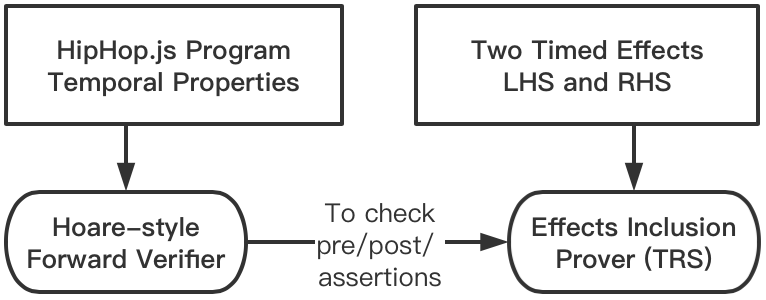
\includegraphics[width=0.5\columnwidth]{verification.png}
        \vspace{-3mm}
\caption{\label{fig:Verification_oberview}System Overview.}
      \vspace{-1mm}
\end{wrapfigure}

An overview of our automated verification system is given in \figref{fig:Verification_oberview} It consists of a Hoare-style forward verifier and a TRS. 
The inputs of the forward verifier are HipHop.js programs annotated with temporal specifications written in timed synchronous effects (cf. \figref{fig:overview_eg1}). 

The input of the TRS is a pair of effects LHS and RHS, referring to the inclusion LHS \code{\CONTAIN} RHS to be checked 
\textit{(LHS refers to left-hand side effects, and RHS refers to right-hand side effects.)}. Besides, the verifier calls the TRS to prove produced inclusions, i.e., between the effects states and pre/post conditions or assertions (cf. \figref{fig:forward_example}). The TRS will be explained in \secref{sec:Entailment_Prover}. 




In this section, we give an axiomatic semantics model\footnote{Based on the operational semantics of Esterel and JavaScript's asynchrony formally defined in \cite{berry1992esterel} and  \cite{madsen2017model} respectively.} for the core language \code{\lambda_{HH}}, by formalising a set of forward inductive rules. 
These rules transfer program states and systematically accumulate the effects syntactically. 
To define the model, we introduce an environment \env\ and describe a program state in a four-elements tuple \code{\langle \Pi, H, C, T \rangle}, with the following concrete domains:
\begin{flalign*}
\Pi {\defeq} t {\rightarrow} \pi, \qquad
H  {\defeq} es, \qquad
C {\defeq} \overrightarrow{\textbf{S} {\rightarrow} \Delta}\  | \ \textbf{S}?, \qquad
T {\defeq} t, \qquad 
\env {\defeq} \overrightarrow{\textbf{S}}, \qquad
\Delta {\defeq} \m{Present} \ | \ \m{Absent}  \ | \  \m{Undef}
\end{flalign*}

Let \code{\Pi} represents the pure constraints for all the terms; \code{H} represents the trace of \emph{history}; \code{C} represents the \emph{current} time instance or a waiting signal; 
\code{T} is a term binding \code{C}; 
\env\ be the environment containing all the local and output signals; 
\code{\Delta} marks the signal status. 



%We describe the input and output histories of ESTEREL programs by streams carrying sets of signals.

%which is used for the description of a reactive program. 

%The main difficulty in giving a semantics to \code{\lambda_{HH}} consists in the idea of instantaneous reactions of ESTEREL programs to input signals. 

%We base this semantics on a functional model of behaviour. We describe the input and output histories of ESTEREL programs by streams carrying sets of signals.


%we mainly present the forward verifier
% based on the syntax of each statement. 

%We present the intermediate representation of program states in \figref{fig:intermediate_representation}




%\noindent   the second element represents the  containing the path constraints (\code{\pi}) and signal assignments (\code{\phi})\footnote{The difference between \code{\textbf{S} = \theta} and \code{\textbf{S} \mapsto \theta } is: the former one denotes the constraints along the execution path, which creates \emph{false} if there are two different status assignments to the same signal; while the latter one records the current status of one signal, and will be overwritten when the presence of a signal had been determined.}; 




\subsection{Forward Inference Rules}
\label{Forward_Rules}
To help with reasoning logical errors (cf. \secref{subsec:LogicalIncorrectCatching}), the rule \code{[FV\text{-}Nothing]} extends the current time instance with all the signals in the environment pointing to absent. 
%is the Esterel equivalent of unit, void or skip in other languages, 
% obtains the next program state by inheriting the current program state.
\begin{flalign*}
%%%%%%%%%%%%%%%%%%%%%%%%%%%%
%%                          NOTHING                              %%
%%%%%%%%%%%%%%%%%%%%%%%%%%%%
&\code{\frac{
%\forall \textbf{S} \in \env.\  C[ \textbf{S}\mapsto  Absent]
C^\prime {=} \{\textbf{S}\mapsto  Absent\ |\  \forall \textbf{S} \in \env\}
}{\env \vdash \langle \Pi, H, C, T \rangle\  nothing \ \langle
 \Pi, H, C {+}{+} C^\prime, T \rangle}\ [FV\text{-}Nothing]} 
\end{flalign*}
The rule \code{[FV\text{-}Emit]} extends the current time instance with signal {\textbf{S}}  pointing to \code{Present}. %status of signal \code{\textbf{S}} (from \code{Undef}) to \code{Present}; keeps the pure constraints, the history trace and the current term unchanged.
\begin{flalign*}
%%%%%%%%%%%%%%%%%%%%%%%%%%%%
%%                              EMIT                                 %%
%%%%%%%%%%%%%%%%%%%%%%%%%%%%
&
\code{\frac{
C^\prime {=} C {+}{+} [ (\textbf{S}\mapsto  Present)]
}{\env \vdash \langle \Pi, H, C, T \rangle\  emit \ \textbf{S} \ \langle  \Pi, H, C^\prime, T \rangle}\ [FV\text{-}Emit] } 
\end{flalign*}
The rule \code{[FV\text{-}Yield]} archives the current time instance to the history trace; then initializes a new time instance where all the signals from \code{\env} are set to be undefined. Then the new \emph{current} is bound with a fresh non-negative term \code{ T^\prime}.
\begin{flalign*}
%%%%%%%%%%%%%%%%%%%%%%%%%%%%
%%                            PAUSE                                %%
%%%%%%%%%%%%%%%%%%%%%%%%%%%%
&
\code{\frac{
\Pi^\prime {=} \Pi \wedge  T^\prime {\geq}0 \qquad 
C^\prime {=} \{\textbf{S}\mapsto  Undef\ |\  \forall \textbf{S} \in \env\} \qquad
H^\prime {=} H \cdot (C\# T) \qquad
( T^\prime\ is\ fresh)
}{\env \vdash 
\langle  \Pi, H, C, T  \rangle\  yield \ \langle 
 \Pi^\prime, H^\prime, C^\prime,  T^\prime \rangle}\ [FV\text{-}Yield]} 
\end{flalign*}


The rule \code{[FV\text{-}Present]} 
enters into branches \code{p} and \code{q} after setting the status of  {\textbf{S}} in the current time instance to \code{Present} and \code{Absent} respectively. We deploy the \code{cut} function to reallocate the next program state. {Each signal can be reset from \code{\m{Undef}} to \code{\m{Present}} or \code{\m{Absent}} maximum once.}
\begin{flalign*}
%%%%%%%%%%%%%%%%%%%%%%%%%%%%
%%                          PRESENT                              %%
%%%%%%%%%%%%%%%%%%%%%%%%%%%%
&
\code{\frac{
\begin{matrix}
\text{\code{
 \env \vdash \langle  \Pi, H, C[ \textbf{S}\mapsto  Present], T  \rangle\  {p} \ \langle 
 \Pi_1, H_1, C_1,  T_1 
 \rangle
}}\\
 \text{\code{
\env \vdash \langle  \Pi, H, C[ \textbf{S}\mapsto  Absent], T  \rangle\  {q} \ \langle 
 \Pi_2, H_2, C_2,  T_2 
\rangle 
}}
\\
 \text{
\code{
\langle   \Pi^\prime , H^\prime, C^\prime,  T^\prime \rangle {=} cut \ (\Pi_1 \wedge \Pi_2 : H_1 \cdot (C_1\#T_1) \vee H_2 \cdot (C_2\#T_2) )
} 
 }
\end{matrix}
}{\env \vdash \langle  \Pi, H, C, T  \rangle\  present \ \textbf{S} \ {p} \ {q}  \ \langle  \Pi^\prime, H^\prime, C^\prime,  T^\prime \rangle}\ [FV\text{-}Present] } 
\end{flalign*}
}
%Intuitively, Cut is defined in, with the intuition of cutting a trace es into a history trace H and a current time instance \code{C\#T}.
\begin{definition}[Cut]\label{Def_cut} 
Given any \code{\pi} and \code{\es}, we define: 
\code{cut(\pi{:} \es)} computes \code{\langle \Pi, H, C, T \rangle. 
} In particular, 
{ 
\begin{gather*}
\code{cut(\pi:\es^\prime \cdot I){=} \langle \pi\wedge T{\geq}0, \es^\prime, I, T \rangle}    \qquad  (\es{=}\es^\prime \cdot I, \ T\ is\ \m{fresh})
\\
 \code{cut(\pi:(\es^\prime \cdot I) \# t) {=} \langle \pi\wedge T_1{\geq}0\wedge T_2{\geq}0 \wedge T_1{+}T_2{=}t, \es^\prime \#T_1, I, T_2 \rangle} \quad \ 
 (\es{=}(\es^\prime \cdot I)\# t, \ T_1, \ T_2 \ are\ \m{fresh})
\end{gather*}}
\end{definition}

The rule \code{[FV\text{-}Fork]} gets \code{\langle \Pi_1, H_1, C_1, k_1   \rangle} and 
\code{\langle \Pi_2, H_2, C_2, k_2 \rangle} by executing \code{{p}} and \code{{q}} independently. 
We parallel synchronise the effects from these two branches; and use the \code{cut} function to reallocate the next program state. 
\begin{flalign*}
&
%%%%%%%%%%%%%%%%%%%%%%%%%%%%
%%                             PAR                                %%
%%%%%%%%%%%%%%%%%%%%%%%%%%%%
\code{\frac{
\begin{matrix}
\text{\code{
\env \vdash \langle  \Pi, H, C, T  \rangle\  {p} \ \langle  \Pi_1, H_1, C_1, T_1 
 \rangle 
}}\qquad\quad
 \text{\code{
\env \vdash \langle  \Pi, H, C, T  \rangle\  {q} \ \langle \Pi_2, H_2, C_2, T_2 
\rangle 
 }}\\
 \text{\code{
\langle \Pi^\prime, H^\prime, C^\prime,  T^\prime \rangle {=} cut\ (
\Pi_1 \wedge \Pi_2 :  H_1 \cdot (C_1\#T_1) \ || \ H_2 \cdot (C_2\#T_2))
 }}
\end{matrix}
}{\env \vdash \langle  \Pi, H, C, T  \rangle\  fork\  {p}  \ {q} \ \langle   \Pi^\prime , H^\prime, C^\prime,  T^\prime \rangle} \ [FV\text{-}Fork] } 
\end{flalign*}
The rule \code{[FV\text{-}Seq]} firstly gets \code{ \langle \Pi_1, H_1, C_1, T_1  \rangle} by executing \code{{p}}. Then it further gets  \code{ \langle \Pi_2, H_2, C_2, T_2 \rangle}  by continuously executing \code{{q}}, to be the final program state.
%and returns \code{\effect_1^{k_1}} to be the final effects. 
%the rule splits \code{\effect_1} into \code{\tau^{\prime}} and  \code{ (\Pi^\prime {\wedge}  \phi^\prime )}; constructs the final effect \code{\effect_2^{k_2}} by  executing \code{\textbf{p}_2}.
\begin{flalign*}
%%%%%%%%%%%%%%%%%%%%%%%%%%%%
%%                             SEQ                                %%
%%%%%%%%%%%%%%%%%%%%%%%%%%%%
&
\code{\frac{
\begin{matrix}
\text{\code{
\env \vdash \langle  \Pi, H, C, T  \rangle\  {p} \ \langle  \Pi_1, H_1, C_1, T_1 
 \rangle 
}}\qquad\quad
 \text{\code{
\env \vdash \langle \Pi_1, H_1, C_1, T_1  \rangle\  {q} \ \langle \Pi_2, H_2, C_2, T_2 
\rangle 
 }}
\end{matrix}
}{\varrho \vdash \langle \Pi, H, C, T \rangle \  seq\  {p} \ {q}  \ \langle \Pi_2, H_2, C_2, T_2 
\rangle  }\ [FV\text{-}Seq]  } 
\end{flalign*}


The rule \code{[FV\text{-}Loop]} computes a fixpoint (as the invariant effects of the loop body) \code{\langle \Pi_2, H_2, C_2, T_2 \rangle} by continuously executing \code{p} twice\footnote{The deterministic loop invariant can be fixed after the second run of the loop body, cf. \appref{proof:twice} for the proof.}, starting from temporary initialised program states \code{\langle \Pi, \empt,  C , T \rangle} and 
\code{\langle \Pi_1, \empt,  C_1 , T_1  \rangle} respectively. 
The final state will contain a repeated trace \code{(H_2 \cdot C_2\# T_2 )^\star}.
% Then anything following an infinite trace will be abandoned. (cf. \tabref{table:normalization})
%gets \code{\langle\effect^k \rangle} by initializing the precondition with \code{\empt} to be the history trace and the current instant by mapping all the local signals to \code{absent} before executing \code{ \textbf{p}}. When there is no exit from the loop body (\code{k{=}0}), the final effects is an infinite trace constructed by \code{(\tau \cdot (\Pi \wedge  \phi) \cdot \effect^\omega)^0}. Otherwise, when there is an exit in the loop body, the final effects is a finite trace \code{(\tau \cdot (\Pi \wedge  \phi) \cdot \effect)^k}, reflecting the completion code \code{k}.
\begin{flalign*}
%%%%%%%%%%%%%%%%%%%%%%%%%%%%
%%                             LOOP                                %%
%%%%%%%%%%%%%%%%%%%%%%%%%%%%
&
\code{\frac{
\begin{matrix}
\text{\code{
\env \vdash  \langle \Pi, \empt,  C , T  \rangle\  {p} \ \langle \Pi_1, H_1, C_1, T_1 \rangle \qquad\quad 
\env \vdash  \langle \Pi_1, \empt,  C_1 , T_1  \rangle\  {p} \ \langle \Pi_2, H_2, C_2, T_2\rangle  
 }}\\
 \text{
\code{
H^\prime {=} H \cdot H_1 \cdot (H_2 \cdot C_2\# T_2 )^\star \cdot H_2
} 
 }
 %\qquad \code{C^\prime = \{\textbf{S}\mapsto  absent\ |\  \forall \textbf{S} \in \varrho\}}
\end{matrix}
}{\env \vdash \langle \Pi, H, C, T \rangle\  loop \ {p} \ \langle  \Pi_2, H^\prime, C_2 , T_2 \rangle} \ [FV\text{-}Loop]} 
\end{flalign*}

%The rule \code{[FV\text{-}Trap]} gets \code{\langle \Pi^\prime, H^\prime, C^\prime, k^\prime \rangle} by executing the trap body \code{ \textbf{p}}.
%When there is no exit from the trap body (\code{k{=}0}), or there is an exit which can be exactly catched by the current trap (\code{k{=}1}), we leave the final completion code to be 0. When there is an exit with a higher priority, (\code{k{>}1}), indicating to exit from a outer trap, we get the final \code{k_f} by decreasing  the completion code by one.  

%\begin{flalign*}
%%%%%%%%%%%%%%%%%%%%%%%%%%%%%
%%%                             TRAP                                %%
%%%%%%%%%%%%%%%%%%%%%%%%%%%%%
%&
%\code{\frac{
%\begin{matrix}
%\text{\code{
% \env \vdash \langle \Pi, H, C, k  \rangle\  \textbf{p} \ \langle \Pi^\prime, H^\prime, C^\prime, k^\prime 
%   \rangle
% }}\\
% \text{\code{
%k_f  = 0  \qquad\qquad\   when \quad k^\prime {\leq} 1 }}\\
%\text{\code{
%k_f  = k^\prime\text{-}1  \qquad\quad\   when \quad k^\prime {>} 1 }}
%\end{matrix}
%}{\env \vdash \langle \Pi, H, C, k  \rangle\  trap\ \textbf{T} \ \textbf{p} \ \langle   \Pi^\prime, H^\prime, C^\prime, k_f \rangle}\ [FV\text{-}Trap]} 
%\end{flalign*}
%
%As \code{exit \ \textbf{T}_{k^\prime}} will abort execution up to the \code{(k^\prime{+}1)}th enclosing of the trap \code{\textbf{T}}.
%%reducing it to nothing. It can be used for exception handling, but also for non-exceptional control flow. 
%The rule \code{[FV\text{-}Exit]} sets the value of \code{k} using \code{k^\prime{+}1}. %and keeps the history trace and the current time instant unchanged. 
%\begin{flalign*}
%%%%%%%%%%%%%%%%%%%%%%%%%%%%%
%%%                             EXIT                                %%
%%%%%%%%%%%%%%%%%%%%%%%%%%%%%
%&
%\code{\frac{
%}{\env \vdash \langle \Pi, H, C, k \rangle\  exit \ \textbf{T}_{k^\prime} \  \langle  \Pi, H, C, k^\prime{+}1 \rangle}\ [FV\text{-}Exit]} 
%\end{flalign*}
%
The rule \code{[FV\text{-}Call]} triggers the back-end solver TRS to  check if the precondition of the callee, \code{\effect_{pre}}, is satisfied by the current effects state or not. If it holds, the rule obtains the next program state by concatenating the postcondition \code{\effect_{post}} to the current effects state. (cf. \figref{fig:forward_example}) 
\begin{flalign*}
&
\code{\frac{
\begin{matrix}
\code{nm  \ \ {(\overrightarrow{\tau\ x}, \  \overrightarrow{\tau\ \textbf{S}} )}\ \langle\textbf{requires}\  \effect_{pre}\ \ \textbf{ensures}\ \effect_{post} \rangle\ {p} \in \mathcal{P}}\\
\code{\textit{TRS}  \vdash  \Pi : H \cdot (C\# T)  \CONTAIN \effect_{pre} }
\qquad\quad
\code{
\langle \Pi^\prime, H^\prime, C^\prime,  T^\prime \rangle {=} cut\ (\Pi :  H \cdot (C\#T) \cdot \effect_{post})
}
\end{matrix}
}{\env \vdash \langle \Pi, H, C, T \rangle\  run \ nm \ {( \overrightarrow{x}, \overrightarrow{ \textbf{S}})} \ \langle \Pi^\prime, H^\prime, C^\prime,  T^\prime \rangle } \ [FV\text{-}Call]  } 
\end{flalign*}

The rule \code{[FV\text{-}Abort]} initialises the state using \code{\langle  \Pi, \epsilon, C, T  \rangle} before entering into \code{ {p}}, and  obtains \code{\langle \Pi^\prime, H^\prime, C^\prime,  T^\prime \rangle} after the execution; then uses a fresh time variable  \code{T_d} to set an upper-bound for the execution \code{H^\prime \cdot (C^\prime \# T^\prime)}, where the constraint on \code{T_d} is \code{0{\leq}T_d{\leq} d}. Lastly, it sets the new current time instance \code{C^{\prime\prime}} by setting all the existing signals to undefined, which is bound with a fresh non-negative term \code{ T_f}.
\begin{flalign*}
%%%%%%%%%%%%%%%%%%%%%%%%%%%%
%%                              ABORT                              %%
%%%%%%%%%%%%%%%%%%%%%%%%%%%%
&
\code{\frac{
\begin{matrix}
\text{
\code{
\env \vdash \langle  \Pi, \epsilon, C, T  \rangle\   {p} \ \langle \Pi^\prime, H^\prime, C^{\prime},  T^\prime  \rangle
\qquad\quad
\Pi^{\prime\prime} {=} \Pi^{\prime} \wedge (0 {\leq}T_d{<} d) \wedge (T_f {\geq}0)
}}
 \\
\text{
\code{
H^{\prime\prime} {=} (H^\prime \cdot (C^{\prime}\#  T^\prime)) \# T_d
}}\qquad
\text{\code{
C^{\prime\prime} {=} \{\textbf{S}\mapsto  \m{Undef}\ |\  \forall \textbf{S} \in \env\}
\qquad\quad \m{(T_d, T_f\ are\ fresh)}
}}
\end{matrix}
}{\env \vdash \langle \Pi, H, C, T \rangle\  abort\ {p}\ when\ d \ \langle \Pi^{\prime\prime}, H\cdot H^{\prime\prime}, C^{\prime\prime}, T_f  \rangle} \ [FV\text{-}Abort]} 
\end{flalign*}

Dually, the rule \code{[FV\text{-}Async]} initialises the states using \code{\langle  \Pi, \epsilon, C, k  \rangle} before entering into \code{ {p}}, and  obtains \code{\langle \Pi^\prime, H^\prime, C^\prime, k^\prime \rangle} after the execution; then uses a fresh time variable  \code{T_d} to set a lower-bound for the execution \code{H^\prime \cdot (C^{\prime} \# T^\prime)}, where the constraint on \code{T_d} is \code{T_d{\geq} d}. Lastly, it creates the new current time instance  \code{C^{\prime\prime}}  by
setting \textbf{S} to present instantaneously, and the rest of the signals in \code{\env}  to undefined (as it emits \textbf{S} once the asynchronous execution is completed), which is bound with a fresh non-negative term \code{ T_f}.
%[ \textbf{S} \mapsto  present]
\begin{flalign*}
%%%%%%%%%%%%%%%%%%%%%%%%%%%%
%%                              ASYNC                              %%
%%%%%%%%%%%%%%%%%%%%%%%%%%%%
&
\code{\frac{
\begin{matrix}
\text{\code{\env \vdash \langle  \Pi, \epsilon, C, T  \rangle\   {p} \ \langle \Pi^\prime, H^\prime, C^{\prime},  T^\prime  \rangle
\qquad\quad \m{(T_d, T_f\ are\ fresh)}
}}
 \\
\text{
\code{
\Pi^{\prime\prime} {=} \Pi^{\prime} \wedge (T_d{\geq} d)  \wedge (T_f {\geq} 0)
\qquad \qquad
H^{\prime\prime} {=}  (H^{\prime} \cdot (C^{\prime}\#  T^\prime)) \# T_d
}}\\
\text{\code{
C^{\prime\prime} {=} \{\textbf{S}^\prime \mapsto  \m{Undef}\ |\  \forall \textbf{S}^\prime \in (\env \symbol{92} \textbf{S}) \} \cup \{ \textbf{S} \mapsto  Present\}
}}
\end{matrix}
}{\env \vdash \langle \Pi, H, C, T \rangle\  async\ \textbf{S} \ {p} \  d \  \langle \Pi^{\prime\prime}, H \cdot H^{\prime\prime}, C^{\prime\prime}, T_f \rangle}\ [FV\text{-}Async]} 
\end{flalign*}

The rule \code{[FV\text{-}Await]} archives the current time instance to the history trace, then sets a new current instance as a waiting for signal {\textbf{S}}, bound with a fresh non-negative term \code{ T^\prime}.
%updates the current status of signal \code{\textbf{S}} to \code{waiting}; keeps the pure constraints, history trace and completion code unchanged.
\begin{flalign*}
%%%%%%%%%%%%%%%%%%%%%%%%%%%%
%%                              AWAIT                                 %%
%%%%%%%%%%%%%%%%%%%%%%%%%%%%
&
\code{\frac{
\Pi^\prime {=} \Pi \wedge  T^\prime {\geq}0 \qquad  
H^\prime {=} H \cdot (C\# t) \qquad ( T^\prime\ is\ fresh)
}{\env \vdash \langle \Pi, H, C, T \rangle\  await \ \textbf{S} \ \langle  \Pi^\prime, H^\prime, \textbf{S}?,  T^\prime \rangle}\ [FV\text{-}Await] } 
\end{flalign*}



The rule \code{[FV\text{-}Assert]} simply checks if the asserted property \code{\effect} is satisfied by the current effects state. If not, a compilation error will be raised. 
\begin{flalign*}
&
\code{\frac{
\begin{matrix}
\code{\textit{TRS}  \vdash  \Pi \wedge (H \cdot (C\#T ) \CONTAIN \effect }
\end{matrix}
}{\env \vdash \langle \Pi, H, C, T  \rangle\  assert\ \effect  \ \langle \Pi, H, C, T  \rangle}\ [FV\text{-}Assert]} 
\end{flalign*}



     






\section{Temporal Verification via a TRS}
\label{sec:Entailment_Prover}


The TRS  is an automated entailment checker to prove language inclusions among timed synchronous effects (cf. \defref{Inclusion} and \tabref{tab:rewriting_tree_send}). It is triggered i) prior to temporal property assertions; ii) prior to module calls for the precondition checking; and iii) at the end of verifying a module for the post condition checking. Given two effects \code{\effect_1,\ \effect_2}, TRS decides if the inclusion \code{\effect_1 \CONTAIN  \effect_2 } is valid. 

During the effects rewriting process, the inclusions are in the form of \code{\Gamma \vdash  \effect_1 \CONTAIN^{\effect}  \effect_2 }, a shorthand for: \code{\Gamma \vdash  \effect \cdot \effect_1 \CONTAIN   \effect \cdot  \effect_2}. To prove such inclusions is to check whether all the possible timed traces in the antecedent \code{\effect_1} are legitimately allowed  in the possible timed traces from the consequent \code{\effect_2}.
\code{\Gamma} is the proof context, i.e., a set of effects inclusion hypothesis, \code{\effect} is the history effects from the antecedent that have been used to match the effects from the consequent.
Note that \code{\Gamma}, \code{\effect} are derived during the inclusion proof. 
The inclusion checking is initially invoked with \code{\Gamma{=}\{\}} and \code{\effect{=} True : \empt}. 







\paragraph{\textbf{Effects Disjunctions.}}
An inclusion with a disjunctive antecedent succeeds if both disjunctions entail the consequent.  An inclusion with a disjunctive consequent succeeds if the antecedent entails either of the disjunctions.  
{ 
 \begin{gather*}
\frac{ \begin{matrix}
    \text{\code{\Gamma \vdash  \effect_1 \CONTAIN  \effect  \qquad \Gamma \vdash \effect_2 \CONTAIN  \effect}}
  \end{matrix}}{\Gamma \vdash  \effect_1 \vee \effect_2 \CONTAIN  \effect}\  \code{[LHS\text{-}OR]}
\qquad
\frac{ \begin{matrix}
    \text{\code{\Gamma \vdash  \effect \CONTAIN  \effect_1  \quad or \quad \Gamma \vdash \effect \CONTAIN  \effect_2}}
  \end{matrix}}{\Gamma \vdash    \effect \CONTAIN \effect_1 \vee \effect_2}\  \code{[RHS\text{-}OR]}
\end{gather*}



}

Now, the inclusions are disjunction-free formulas. 
Next we provide the definitions and implementations of auxiliary functions \emph{Nullable}(\code{\delta}), \emph{First}(\code{fst}) and \emph{Derivative}(\code{D}) respectively.
Intuitively, the Nullable function \code{\delta(\es)} returns a boolean value indicating whether \code{\es} contains the empty trace; the First function \code{fst_{\pure{\pi}}( \es)} computes a set of possible initial time instances of \code{\pure{\pi} : \es}; and the Derivative function \code{D_{I\# t}^{\pure{\pi}}(\es)} computes a next-state effects after eliminating one time instance \code{I} w.r.t. the execution time \code{t} from the current effects \code{\pure{\pi} : \es}. 



%\subsection{closure of clock constrains}
%how to eliminate the unobservable transitions. 
%
%we allow the $\empt$transitions without carrying constraints and resetting clocks at the same time. 




\begin{definition}[Nullable]\label{Nullable}
Given any time sequence \code{\es}, we recursively define \code{\delta(\es)} as:\\
{
\code{\delta(\es) :bool {=}
\begin{cases}
      \code{true} & \code{if\ \empt \in \es}\\
      \code{false} & \code{if\ \empt \notin \es}
    \end{cases} }
    }, where   
{ 
\begin{gather*}
\code{\delta(\bott) {=} false} 
\qquad\quad
\code{\delta(\empt) {=} true} 
\qquad\quad
\code{\delta(I){=} false}   
\qquad\quad
\code{\delta(\textbf{S}?){=} false}   
\qquad\quad\
    \code{\delta(\esn{\es}{\star} ) {=} true}   
\\ 
\code{\delta(\es_1 \seq \es_2) {=} \delta(\es_1) \wedge \delta(\es_2)}
\qquad\qquad
  \code{\delta(\es_1 \choice \es_2) {=} \delta(\es_1) \vee \delta(\es_2)}   
  \qquad\quad
  \code{\delta(\esn{\es}{\omega} ) {=} false}     
  \\
\code{\delta(\es_1 || \es_2) {=} \delta(\es_1) \wedge \delta(\es_2)}
\qquad\qquad\quad
 \code{\delta(\es \# t) {=} \delta(\es)}
\end{gather*}}
\end{definition}

To better outline our contribution, we first present the original \emph{First} function used in  Antimirov's rewriting system, denoted using \code{fst^\prime}, defined as follows:

\begin{definition}[Antimirov's First]\label{First1}
Let \code{fst^\prime(\es){:=}\{ I\ |\  (I \cdot \es^\prime) \in \llbracket  \es \rrbracket  \}} be the set of initial instances derivable from  sequence \code{\es}. (\code{\llbracket  \es \rrbracket } represents all the traces contained in \code{\es}.)
{ 
 \begin{gather*} 
\code{fst^\prime( \bott) {=} \{ \} } \qquad\ 
\code{ fst^\prime(\empt) {=} \{ \}} \qquad\ 
\code{fst^\prime( I) {=} \{ I \} }
 \qquad\ 
\code{fst^\prime(  \es_1 {\vee} \es_2) {=} fst^\prime(  \es_1) \cup fst^\prime(  \es_2)}
\\
{
\code{fst^\prime( \esn{\es}{\star} ) {=} fst^\prime({ \es})} 
\qquad\quad\
\code{fst^\prime(\es_1 {\seq} \es_2) {=} } 
\begin{cases}
      \code{\code{fst^\prime(  \es_1)} \cup \code{fst^\prime(  \es_2)} } \quad & \code{ if\ \delta(\es_1) {=} true}\\
      \code{\code{fst^\prime(  \es_1)}} & \code{  if\ \delta(\es_1) {=} false}
    \end{cases} 
    }
\end{gather*}
}
\end{definition}

As shown, \code{fst^\prime} does not handle 
%the concurrent operator \code{||} nor contains 
any arithmetic constraints, nor 
the real-time bounds constructor \code{\#}. Next, we define the novel  \emph{First} function used in this work, denoted using \code{fst}. 
%but helps to build up our \emph{First} function \code{fst}. 

\begin{definition}[First]\label{First}
Let \code{fst_{\pure{\pi}}(\es){:=}\{ (I,  \pi, t) \ |\  \pi {\wedge} t{\geq}0 : (I\# t) \cdot \es^\prime \in \llbracket  \pi {:} \es \rrbracket \}} be the set of initial time instances derivable from effects \code{\pi {:} \es}. (\code{\llbracket  \pi {:} \es \rrbracket } represents all the time  traces contained in \code{\pi {:} \es}) 
{ 
 \begin{gather*} 
\code{fst_{\pure{\pi}}( \bott) {=} \{ \} } \qquad\quad
\code{fst_{\pure{\pi}}(\empt) {=} \{ \} } \qquad\quad
\code{fst_{\pure{\pi}}( I ) {=} \{ (I, \pi {\wedge} t{\geq}0, t) \}  \ (t\ is\ fresh)} 
\qquad\quad
   \code{fst_{\pure{\pi}}(  \es \# t) {=}  fst_{pi}(\es)}
 \\
\code{fst_{\pure{\pi}}( \esn{\es}{\star} ) {=} fst_{\pure{\pi}}({ \es})}
\qquad\quad
\code{fst_{\pure{\pi}}( \esn{\es}{\omega} ) {=} fst_{\pure{\pi}}({ \es})} 
\qquad\quad
\code{fst_{\pure{\pi}}(  \es_1 {\vee} \es_2) {=} fst_{\pure{\pi}}(  \es_1) \cup fst_{\pure{\pi}}(  \es_2)  }  \\
\code{fst_{\pure{\pi}}( \textbf{S}? ) {=} fst_{\pure{\pi}}( \{\textbf{S}\} ) \cup fst_{\pure{\pi}}( \{ \overline{\textbf{S}} \} ) }
    \qquad\qquad\quad
   \code{fst_{\pure{\pi}}(  \es_1 {||} \es_2) {=} unify \ 
    (fst_{\pure{\pi}}(  \es_1)) \  (fst_{\pure{\pi}}(  \es_2))  }  
   \\
{
\code{fst_{\pure{\pi}}(\es_1 {\seq} \es_2) {=} } 
\begin{cases}
      \code{\code{fst_{\pure{\pi}}(  \es_1)} \cup \code{fst_{\pure{\pi}}(  \es_2)} } & \code{ if\ \delta(\es_1) {=} true}\\
      \code{\code{fst_{\pure{\pi}}(  \es_1)}} & \code{  if\ \delta(\es_1) {=} false}
    \end{cases} 
    }  
\end{gather*}
}
\end{definition}


\begin{definition}[First-Tuples Unification]\label{unify} Given two first tuples \code{(I_1, \pi_1, t_1)} and \code{(I_2, \pi_2, t_2) }, we define that: 
%We deploy a \code{unify} function to merge two time instances, where \\ 
\code{unify\ (I_1, \pi_1, t_1)\  (I_2, \pi_2, t_2) = (I_1 \cup I_2, \pi_1 \wedge \pi_2 \wedge (t1 {=} t2), t_1)}.
\end{definition}


\begin{definition}[Instances Subsumption]\label{Subsumption}
Given two instances \code{I} and \code{J}, we define the subset relation \code{I {\subseteq} J} as: the set of present signals in \code{J} is a subset of the set of present signals in \code{I}, and the set of absent signals in \code{J} is a subset of the set of absent signals in \code{I}\footnote{As in having more constraints refers to a smaller set of satisfying instances.}.
Formally, 
 \begin{gather*} 
 \code{I {\subseteq} J \Leftrightarrow  \{\textbf{S}\ |\ (\textbf{S} {\mapsto} Present) \in J \}  \subseteq  \{\textbf{S}\ |\ (\textbf{S} {\mapsto} Present) \in I \}} \\
  \code{ \quad\  and  \ 
 \{\textbf{S}\ |\ (\textbf{S} \mapsto Absent) \in J \}  \subseteq  \{\textbf{S}\ |\ (\textbf{S} \mapsto Absent) \in I \}
 }
\end{gather*}

\end{definition}


\begin{definition}[Time Instances Subsumption]\label{Subsumption1}
Given two time instances \code{(I, \pi_1, t_1)} and \code{(J, \pi_2, t_2)}, we define the subset relation \code{(I, \pi_1, t_1) {\subseteq} (J, \pi_2, t_2)} as:  \code{I {\subseteq} J} and \code{\pi_1[t_2/t_1]  {\Rightarrow}   \pi_2  }.

\end{definition}

\begin{definition}[Partial Derivative\footnote{Intuitively, the partial derivative refers to the left quotient of a language equation, for example, for REs, \code{x^{{-}1} \llbracket x\cdot y\rrbracket {=} y};  \code{y^{{-}1} \llbracket x\cdot y\rrbracket {=} \bott}; and  \code{y^{{-}1} \llbracket x + y\rrbracket {=} \epsilon}. Here we come up with a new notion of partial derivative for timed synchronous effects. 
}]\label{Derivative}
The partial derivative \code{D^{\pi}_{(I, \pi^\prime, t^\prime)}(\es)} 
of effects \code{\pi : \es} 
w.r.t. a time instance \code{(I, \pi^\prime, t^\prime)} computes the  effects for the left quotient \code{(I, \pi^\prime, t^\prime)^{\text{-}1}\llbracket \pi : \es \rrbracket}. \footnote{For understanding of the derivative rule for \code{es\# t} (cf. \tabref{tab:rewriting_tree_send}  step \textcircled{3}), it is essentially splitting \code{\es} with a head and a tail, bound with fresh terms \code{t_1} and \code{t_2} respectively. Meanwhile it unifies \code{t_1} with \code{t^\prime} and  adds the constraint \code{t_1 {+} t_2 {=} t}.}
%\footnote{As the reader may notice, our First and Derivative function does not handle the timed sequences constructed by \code{||}, as the synchronous parallel is reduced during the normalization phase.}
\begin{gather*}
\code{D^{\pi}_{(I, \pi^\prime, t^\prime)}(\bott) {=}}  
 \code{False : \bott} 
\qquad\ 
\code{D^{\pi}_{(I, \pi^\prime, t^\prime)}(  \empt) {=}}   
\code{False : \bott} 
\qquad \ 
\code{D^{\pi}_{(I, \pi^\prime, t^\prime)}(es_1 || es_2)} {=} \code{D^{\pi}_{(I, \pi^\prime, t^\prime)}(es_1)} || \code{D^{\pi}_{(I, \pi^\prime, t^\prime)}( es_2)} 
    \\
        \code{D^{\pi}_{(I, \pi^\prime, t^\prime)}(  \esn{\es}{\star}) } {=} \code{ D^{\pi}_{(I, \pi^\prime, t^\prime)}(  {\es}) \cdot (\esn{\es}{\star})}  
        \qquad\qquad
                \code{D^{\pi}_{(I, \pi^\prime, t^\prime)}(  \esn{\es}{\omega}) } {=} \code{ D^{\pi}_{(I, \pi^\prime, t^\prime)}(  {\es}) \cdot (\esn{\es}{\omega})}  
\\
{
 \code{D^{\pi}_{(I, \pi^\prime, t^\prime)}(   \es_1 \seq \es_2) {=} }
\begin{cases}
      \code{D^{\pi}_{(I, \pi^\prime, t^\prime)}(   \es_1) \cdot  \es_2 \vee  D^{\pi}_{(I, \pi^\prime, t^\prime)}( \es_2)} \quad &\code{if\ \delta(\es_1) {=} true}   \\
      \code{D^{\pi}_{(I, \pi^\prime, t^\prime)}  ( \es_1) \cdot  \es_2} & \code{if\ \delta(\es_1) {=} false} 
    \end{cases} 
    }
 \\
\code{D^{\pi}_{(I, \pi^\prime, t^\prime)}(  \es_1 \choice \es_2) } {=} \code{ D^{\pi}_{(I, \pi^\prime, t^\prime)}(  \es_1) \choice D^{\pi}_{(I, \pi^\prime, t^\prime)}(  \es_2)} 
%\\
%\code{D^{\pi}_{(I, \pi^\prime, t^\prime)}(  \es_1 \ ||\  \es_2) } {=} \code{ D^{\pi}_{(I, \pi^\prime, t^\prime)}(  \es_1) \ ||\ D^{\pi}_{(I, \pi^\prime, t^\prime)}(  \es_2)} 
\\
\code{D^{\pi}_{(I, \pi^\prime, t^\prime)}(  \es \# t) } {=}
\code{
\pi \wedge(t_1{+} t_2 {=}t) \wedge (t_1{=}t^\prime) : (D^{\pi}_{(I, \pi^\prime, t^\prime)}(\es))\# t_2} \ \ \ 
\code{(fresh \ t_1\ t_2 )}
\\
\code{D^{\pi}_{(I, \pi^\prime, t^\prime)}(\textbf{S}?)} {=} \code{\pi: \empt\ (}\code{ I {\subseteq} \{\textbf{S}\})}
\qquad
\code{D^{\pi}_{(I, \pi^\prime, t^\prime)}(\textbf{S}?)} {=} \code{\pi: \textbf{S}?\ (}\code{ I {\not\subseteq} \{\textbf{S}\})}
\\
\code{D^{\pi}_{(I, \pi^\prime, t^\prime)}(J)} {=} \code{\pi: \empt\ (}\code{ I {\subseteq} J)}
\qquad\ 
    \code{D^{\pi}_{(I, \pi^\prime, t^\prime)}( J)} {=} \code{False : \bott \ (}\code{I {\not\subseteq} J)} 
\end{gather*}
\end{definition}




\subsection{Rewriting Rules}
\label{InferenceRules}
Given the well-defined auxiliary functions above, we now discuss the key steps and related rewriting rules that we may use in such an effects inclusion proof.  


\begin{enumerate}
\item 
\textbf{Axiom rules.}
\label{Base}
Analogous to  the standard propositional logic, \code{\bott} (referring to \textit{false}) entails any effects, while no \textit{non-false} effects entails \code{\bott}.
 \begin{gather*}
  \codeme{\frac{
\begin{matrix}
\end{matrix}
}{\text{\code{ \Gamma  \vdash \pi : \bott   \CONTAIN \effect }}}\ [Bot\text{-}LHS]}
\qquad\qquad\quad
\codeme{\frac{
\begin{matrix}
\effect \neq  \pi : \bott 
\end{matrix}
}{\text{\code{\Gamma  \vdash  \effect \not\CONTAIN  \pi : \bott }}} \ \codeme{  [Bot\text{-}RHS]} }
\end{gather*}

\item 
\textbf{Disprove (Heuristic Refutation).}
\label{Refutation}
This rule is used to disprove the inclusions when the antecedent is nullable, while the consequent is not nullable. Intuitively, the antecedent contains at least one more trace (the empty trace) than the consequent. Therefore, the inclusion is invalid. 

\vspace{-4mm}
 \begin{gather*}
\frac{
\begin{matrix}
\text{\codeme{\delta(\es_1) \wedge \neg \delta(\es_2) }}
\end{matrix}
}{\text{\code{\Gamma  \vdash  \pi_1 : \es_1 \not\CONTAIN  \pi_2 : \es_2 }}}\ \codeme{  [DISPROVE]} 
\qquad\ \ 
\frac{
\begin{matrix}
\text{\code{\pi_1 \Rightarrow \pi_2 \quad\ \  
\m{fst}_{\pi_1}(\es_1) = \{\}
%\es_1 \subseteq \es_2 
}}
\end{matrix}
}{\text{\code{\Gamma   \vdash  \pi_1 : \es_1 \CONTAIN  \pi_2 : \es_2 }}}\ \codeme{  [PROVE]} 
\end{gather*}

\item 
\textbf{Prove.}
\label{Prove}
We use two rules to prove an inclusion: (i) \codeme{[PROVE]} is used when the fst set of the antecedent is empty; and (ii) $\code{[REOCCUR]}$ to prove an inclusion
when there exist inclusion hypotheses 
in the proof context $\m{\Gamma}$, which are able to soundly prove the current goal. One of the special cases of this rule is when the identical inclusion is shown in the proof context, we then terminate the procedure and prove it as a valid inclusion. 
 \begin{gather*}
\frac{
\begin{matrix}
\text{\codeme{ (\pi_1 : \es_1 \CONTAIN \pi_3 : \es_3) \in \Gamma  }} 
\quad\ \ 
\text{\codeme{(\pi_3 : \es_3 \CONTAIN  \pi_4 : \es_4) \in {\Gamma} }} \quad\  \ 
\text{\codeme{ (\pi_4 : \es_4 \CONTAIN \pi_2 : \es_2) \in {\Gamma}  }}
\end{matrix}
}{\text{\code{\Gamma  \vdash  \pi_1 : \es_1 \CONTAIN  \pi_2 : \es_2 }} }
\ \codeme{[REOCCUR]}
\end{gather*}

\item 
\textbf{Unfolding (Induction).}
\label{unfolding}
This is the inductive step of unfolding the inclusions. Firstly, we make use of the auxiliary function \code{fst} to get a set of instances \code{F}, which are all the possible initial time instances from the antecedent. 
Secondly, we obtain a new proof context \code{\Gamma^\prime} by adding the current inclusion, as an inductive hypothesis, into the current proof context \code{\Gamma}. 
%(The soundness condition is guaranteed by rule \code{[REOCCUR]} to avoid the possible cyclicity evident in the proof context) 
Thirdly, we iterate each element \code{(I, \pi, t) \in F}, and compute the partial derivatives (\emph{next-state} effects) of both the antecedent and consequent w.r.t \code{(I, \pi, t)}. The proof of the original inclusion succeeds if all the derivative inclusions succeeds.
\begin{gather*}
\frac{ \begin{matrix}
\text{\codeme{F = \m{fst}_{\pure{\pi_1}}(\es_1)\qquad\qquad \Gamma^\prime = \Gamma,  (
\pure{\pi_1} : \es_1 \CONTAIN \pure{\pi_2} : \es_2
)} }\\
    \text{\codeme{\forall (I, \pi, t)\in F. \   (\Gamma^\prime  \vdash \   D_{(I, \pi, t)}^{\pure{\pi_1}}( \es_1) \CONTAIN    D_{(I, \pi, t)}^{\pure{\pi_2}}( \es_2) )}}
  \end{matrix}}
   { \text{\codeme{  \Gamma  \vdash \pure{\pi_1} : \es_1 \CONTAIN \pure{\pi_2} : \es_2 }}}\  \codeme{[UNFOLD]} 
\end{gather*}


\item 
\textbf{Normalization.}
We present a set of normalization rules to soundly transfer the timed effects into a normal form, in particular after getting their derivatives. 
Before getting into the above inference rules, we assume that the effects formulae are tailored accordingly based on the axioms shown in
\tabref{table:normalization}
We built the axiom system on top of a complete axiom system \code{F_1}, from (A1) to (A11), suggested by \cite{salomaa1966two}, which was designed for regular languages. We develop axioms (A12) to (A22) to further accommodate effects constructed by \code{||},   \code{\#} and \code{\omega}.



%\begin{table}[h]
%\vspace{0mm}
%  \caption{Some Normalization Lemmas for timed synchronous effects.}
%  \label{table:normalization}
%\setlength{\tabcolsep}{13pt}
%\renewcommand{\arraystretch}{1.1}
%\centering
%\vspace{0mm}
%\begin{tabular}{l || l || l}
%\hline
%  \code{\es \choice \es \rightarrow \es} 
%  &\code{\bott \cdot \es \rightarrow \bott }  
%  &
% 
%  
%\\ \hline
%
%  \code{\bott \choice \es \rightarrow \es } & \code{ \es  \cdot \bott \rightarrow \bott }  &
%
%\code{ (\es_1 \cdot \es_2) \cdot \es_3 \rightarrow \es_1 \cdot (\es_2 \cdot \es_3)}
%\\ \hline
%
%\code{ \es \choice \bott \rightarrow \es }
%&\code{\bott ^\star \rightarrow \empt}
%& 
%
%
%
%\\ \hline
%
%
% \code{\empt \cdot \es  \rightarrow \es }
% &  \code{\epsilon^\star \rightarrow \epsilon}
% &  
%
% 
%\\ \hline
%
%
%\code{ \es \cdot \empt \rightarrow \es}
%& \code{(\empt \vee \es)^\star \rightarrow \es^\star}
%& \code{ }
%
% 
% 
%\\ \hline
%
%
% 
%
%\\ \hline
%
%\end{tabular}
%\vspace{0mm}
%\end{table}

\begin{table}[h]
\caption{Normalization Axioms for Timed Synchronous Effects.}
\label{table:normalization}
\setlength{\tabcolsep}{10pt}
\renewcommand{\arraystretch}{1.2}
\centering
\begin{tabular}{rl}
\footnotesize

\begin{minipage}[t]{0.4\textwidth}
\begin{tabular}{||l|l}
\hline
(A1)  &
\code{\es_1 \vee (\es_2 \vee \es_3) \rightarrow   (\es_1 \vee \es_2) \vee \es_3 }\\
\hline
(A2)  &
\code{\es_1 \cdot (\es_2 \cdot \es_3)\rightarrow     (\es_1 \cdot \es_2) \cdot \es_3 }\\
\hline
(A3)  &
\code{\es_1 \vee \es_2 \rightarrow   \es_2 \vee \es_1 }\\
\hline
(A4)  &
\code{\es \cdot (\es_1 \vee \es_2)  \rightarrow \es \cdot \es_1  \vee \es \cdot \es_2 }\\
\hline
(A5)  &
 \code{(\es_1 \vee \es_2)\cdot \es   \rightarrow \es_1 \cdot \es   \vee  \es_2 \cdot \es}\\
\hline
(A6)  &
 \code{\es \vee \es   \rightarrow \es}\\
\hline
(A7)  &
 \code{  \es \cdot \epsilon   \rightarrow \es}\\
\hline
(A8)  &
 \code{  \es \cdot  \bot \rightarrow \bot}\\
\hline
(A9)  &
 \code{\es \vee \bot   \rightarrow \es}\\
\hline
(A10)  &
 \code{\epsilon \vee (\es \cdot \es^\star)   \rightarrow  \es^\star}\\
\hline
(A11)  &
 \code{(\epsilon \vee \es)^\star   \rightarrow  \es^\star}\\
\hline



\end{tabular}
  \end{minipage} 
 
  &
\footnotesize
  \begin{minipage}[t]{0.6\textwidth}
\begin{tabular}{||l|l|}
\hline
(A12)  &
\code{\bot^\omega  \rightarrow \bot }\\
\hline
(A13)  &
\code{\es^\omega \cdot \es_1 \rightarrow \es^\omega }\\
\hline
(A14)  &
\code{\epsilon^\omega \rightarrow \bot }\\
\hline
(A15)  &
\code{ \es\ ||\ \empt \rightarrow \es}\\
\hline
(A16)  &
\code{ \es\ ||\ \bott \rightarrow \bott}\\
\hline
(A17)  &
 \code{(I\# t) \cdot \es_1\ ||\ J \cdot\es_2 \rightarrow ((I  {\cup} J) \# t) \cdot (\es_1 || \es_2)}\\
\hline
(A18)  &
\code{\pi : (\es \# t_1 ) \# t_2 \rightarrow \pi  \wedge (t_1 {=} t_2) : \es \# t_1 }\\
\hline
(A19)  &
 \code{\empt \# t \rightarrow \empt}\\
\hline
(A20)  &
 \code{\bot \# t \rightarrow  \bott}\\
\hline
(A21)  &
 \code{{\pure{False}} : \es \rightarrow {\pure{False}} : \bott}\\
\hline
(A22)  &
 \code{{\pi} : \bott \rightarrow {\pure{False}} : \bott}\\
\hline
 %\code{\es \choice \es \rightarrow \es} 
%  &\code{\bott \cdot \es \rightarrow \bott }  
%  &


\end{tabular}
  \end{minipage}
  

 
\end{tabular}
\end{table}



\end{enumerate}






 
\begin{theorem}[Termination]\label{termination}
The rewriting system TRS is terminating.
\end{theorem}
\begin{proof}
See %the technical report\cite{TR}. 
\appref{proof:TerminationProof}.
\end{proof}

 \begin{theorem}[Soundness]\label{Cyclicsoundness}
Given an inclusion \code{\effect_1 \CONTAIN \effect_2}, if the TRS returns \code{TRUE} when proving \code{\effect_1 \CONTAIN \effect_2}, i.e., it has a cyclic proof, 
then \code{\effect_1 \CONTAIN \effect_2} is valid.
\end{theorem}


\begin{proof}
See %the technical report\cite{TR}. 
\appref{proof:SoundnessProof}.
\end{proof}


%\begin{lemma}
%The set of axioms (A1)-(A11) and (A15)-(A22) are complete for timed effects.
%\begin{proof} 
%
%\end{proof}
%\end{lemma}


 \begin{theorem}[Completeness]\label{Completeness}
 The set of axioms (A1)-(A22) is complete for timed synchronous effects.

%Given an inclusion \code{\effect_1 \CONTAIN \effect_2}, if \code{\effect_1 \CONTAIN \effect_2} is valid, then the TRS returns  \code{TRUE} by providing a proof.

\end{theorem}

\begin{proof} 
One can observe that by succinct applications of (A17) to (A22), we have a normal form, 
\begin{align}
\pi_1 : (I\# t_1) \cdot \es_1\ ||\ \pi_2 :  (J\# t_2) \cdot\es_2 \rightarrow  (\pi_1 \wedge \pi_2 \wedge t_1{=}t_2) :  ((I  {\cup} J) \# t_1) \cdot (\es_1\ ||\ \es_2)
\end{align}

Then for any ground timed synchronous effects \code{\es}, the expression \code{\epsilon || \es} can be reduced to either \code{\epsilon} or \code{\es} by the applications of (A15) and (A16).  
The expression \code{\es^\omega} can be reduced to either \code{\bot} or \code{\es^\omega} by the applications of (A12) to (A14).  

Then, by the semantics defined in \figref{fig:Sementic}, effects constructed by Kleene star \code{\star} (possibly finite and possibly infinite) are supersets of effects constructed by \code{\omega} (definite infinite). 

Then one can apply literally all the constructions of \cite{salomaa1966two} used in the completeness proof of \code{F_1} (A1) to (A11).


\end{proof}




\section{Implementation and Case Study}
\label{sec:Evaluation}

\subsection{Implementation}
To show the feasibility of our approach, we have prototyped our automated verification system 
using OCaml \emph{(A demo page  and source code are available from \cite{CODE})}. 
The proof obligations generated by the verifier are discharged using constraint solver Z3 \citep{de2008z3}. 
We prove termination and correctness of the TRS. We validate the front-end forward verifier for conformance, against two implementations: the Columbia Esterel Compiler (CEC) 
\cite{CEC} and Hiphop.js \cite{HH_im}. 


CEC is an open-source compiler designed for research in both hardware and software generation from the Esterel synchronous language to C or Verilog circuit description. It currently supports a subset of Esterel V5, and provides pure Esterel programs for testing. Hiphop.js's implementation facilitates the design of complex web applications by smoothly integrating Esterel and JavaScript, and provides a bench of programs for testing purposes. 



%The core implementation is less than 3500 LOC, roughly, 1000{+} LOC for the verifier, and 2000{+} LOC for the TRS. We prove the soundness of the TRS. 
%Next, we show case studies to demonstrate the feasibilities of our timed synchronous effects comparing to timed automata. 

%We summarize the underlying reasons which lead to the improvement: (1)When the transition states of the models are small, the average execution time spent by the T.r.s is even less than the automata construction time, which means it is not necessary to construct the automata when a TRS solves it faster; (2)When the total states become larger, on average, the TRS outperforms automata-based algorithms, due to the significantly reduced search branches provided by the normalization lemmas; and (3)For the invalid cases, the TRS disproves them earlier without constructing the whole automata.

%\subsubsection{Experimental Setup}~\\

   %   \vspace{-2mm}
   

Based on these two benchmarks, we validate the verifier using 155  programs, varying from 15 lines to 300 lines. We manually annotate temporal specifications in our timed effects, including both succeeded and failed instances (roughly with the a 1:1 ratio). 
Out of the whole test suite, 101 were from the CEC benchmark, 54 were from the Hiphop.js benchmark.  Since async-await was inherited from JavaScript features, it only presents in the 54 hiphop.js programs.
We conduct experiments on a MacBook Pro with a 2.6 GHz Intel Core i7 processor. Given our benchmark, the running time varying from 0 to 500 ms. 

%We claim that the extra expressiveness gained from our logic is the symbolic time-bounds. The timed effects represent not only one exact Timed Automata but also a set of Timed Automata. Together with our back-end inclusion solver, it enables a verification framework for a group of Automata. More specifically, instead of running the model checker many times for one non-deterministic time-bound at each time, we can define arithmetic constraints bounding the time variable. And to test that, we cover a number of test cases with function calls, and the callee's parameters would be used as the time bounds.

Our implementation is the first that solves the  inclusion problem of symbolic timed automata, which is considered important because it overcomes the following main limitations in traditional timed model checking:  i) they cannot be used to specify and verify systems incompletely specified (i. e., whose timing constants are not known yet), and hence cannot be used in early design phases; ii) verifying a system for a set of timing constants usually requires to enumerate all of them one by one if they are supposed to be integer-valued; in addition, timed automata cannot be used to verify a system for a set of timing constants that are to be taken in a real-valued dense interval. 



A term rewriting system is efficient because \emph{it only constructs automata as far as it needed}, which makes it more efficient when disproving incorrect specifications, as we can disprove it earlier without constructing the whole automata. In other words, the more incorrect specifications are, the more efficient our solver is.

%
%\subsubsection{Experimental Results}~\\
%\label{subsec:Experimental_Results}
%
%\begin{table}[h]
%        \vspace{-2mm}
%\caption{\label{tab:Experimental} The experiments are based on 16 real world C programs, we record the lines of code (LOC), the number of testing temporal properties ($\#$Prop.), and the (dis-) proving times (in milliseconds) using PAT and our T.r.s respectively. }
%\centering
%\footnotesize
%\renewcommand{\arraystretch}{1.1}
%\begin{tabular} {l|c|c|c|c}
%\hline
%\textbf{Programs} & \textbf{LOC} & \textbf{$\#$Prop.}  & \textbf{PAT(ms)} & \textbf{T.r.s(ms)} \\ \hline\hline
%1. Chrome\_Dino\_Game    &      80    &    12  &  32.09 &  7.66  \\ \hline
%2. Cradle\_with\_Joystick  &      89     &   12   &  31.22    &   9.85  \\ \hline
%3. Small\_Linear\_Actuator  &    180  &     12  &   21.65      &  38.68  \\ \hline
%4. Large\_Linear\_Actuator &    155   &    12   &  17.41   &   14.66   \\ \hline
%5. Train\_Detect  &                    78   &     12    &   19.50   & 17.35     \\ \hline
%6. Motor\_Control  &                 216  &    15  &     22.89  &  4.71  \\ \hline
%7. Train\_Demo\_2  &                133  &   15    &     49.51   &  59.28   \\ \hline
% 8. Fridge\_Timer  &                  292   &    15   &   17.05   & 9.11 \\ \hline
%  9. Match\_the\_Light   &         143     &    15  &  23.34    &  49.65 \\ \hline
%   10. Tank\_Control  &              104   &    15    &  24.96   &   19.39 \\ 
%     \hline
%  \textbf{\quad \ \ Total}  & 2546    &  235   &  446.88   &   305.33   \\ \hline
%\end{tabular}
%        \vspace{0mm}
%\end{table}
%
%
%        \vspace{-2mm}
%
%
%


\subsection{Case Studies}
\label{subsec:Case_Studies}

Let's recall the existing challenges in different programming paradigms discussed in \secref{sec:Preliminaries}. In this section, we first investigate how our effects logic can help to debug errors related to both synchronous and asynchronous programs. Specifically, it effectively resolves the logical correctness checking (for synchronous languages) and critical anti-patterns checking (for premise asynchrony). 
Meanwhile, we further demonstrate the flexibility and expressiveness of our effects logic. 

%how our proposal makes it flexible for different effects logics.     



\subsubsection{Logical Incorrect Catching}~\\
\label{subsec:LogicalIncorrectCatching}

      \vspace{-2mm}
%We say that the program is logically reactive (resp. logically deterministic) w.r.t. the input event if there is at least (resp. at most) one logically coherent global status. 

%A program is logically correct if there exists precisely \textbf{one} status for each signal that respects the coherence law. 
%it is both logically reactive and deterministic. 
%To effectively check logical correctness, 
We regard these programs, which have precisely one safe trace reacting to each input assignments, as logical correct. 
To effectively check logical correctness, in this work, given a synchronous  program, after been applied to the forward rules, we compute the possible execution traces in a disjunctive form; then prune the traces contain contradictions, following these principles: (i) explicit present and absent; (ii) each local signal should have
only one status; (iii) lookahead should work for both present and absent; (iv) signal emissions are idempotent; (v) signal status should not be contradictory.
Finally, upon each assignment of inputs, programs have none or multiple output traces that will be rejected, corresponding to no-valid or multiple-valid assignments. 


\begin{table}[h]
\centering
\begin{tabular}{c|c|c}
\footnotesize
\begin{minipage}[t]{0.32\textwidth}
\begin{enumerate}
  \item  \code{\key{present}\ S1 } 
  \\
 \code{\langle  \textcolor{darklavender}{true : \{\}} \rangle }
       
  \item    \code{~\qquad \jskey{then}}
   \\
 \code{\langle  \textcolor{darklavender}{true : \{S1\} } \rangle }
   \item    \code{~\qquad~\qquad \key{nothing}}
         \\
 \code{\langle  \textcolor{darklavender}{true : \{S1, \overline{S1}\}} \rangle }
  \item \code{~\qquad  \jskey{else} }
  \\
 \code{\langle  \textcolor{darklavender}{true : \{\overline{S1}\} } \rangle }
  \item    \code{~\qquad~\qquad \key{emit}\ S1 }
     \\
 \code{\langle  \textcolor{darklavender}{true : \{\overline{S1}, S1\}} \rangle }
     \item    \code{  \key{end}\  \key{present} }
     \\
 \code{\langle  \textcolor{darklavender}{true : \{S1, \overline{S1}\} \vee \{\overline{S1}, S1\}} \rangle }
     \\
      \code{\langle  \textcolor{darklavender}{false : \bot} \rangle }
     
     
\end{enumerate}

  \end{minipage} 
 
  &
  \small
  \begin{minipage}[t]{0.32\textwidth}
   \begin{enumerate}
  \item  \code{\key{present}\ S1 } 
  \\
 \code{\langle  \textcolor{darklavender}{true : \{\}} \rangle }
       
  \item    \code{~\qquad \jskey{then}}
   \\
 \code{\langle  \textcolor{darklavender}{true : \{S1\} } \rangle }
  \item    \code{~\qquad~\qquad \key{emit}\ S1 }
     \\
 \code{\langle  \textcolor{darklavender}{true : \{{S1}, S1\}} \rangle }

  \item \code{~\qquad  \jskey{else} }
  \\
 \code{\langle  \textcolor{darklavender}{true : \{\overline{S1}\} } \rangle }
   \item    \code{~\qquad~\qquad \key{nothing}}
         \\
 \code{\langle  \textcolor{darklavender}{true : \{\overline{S1}, \overline{S1}\}} \rangle }
     \item    \code{  \key{end}\  \key{present} }
     \\
 \code{\langle  \textcolor{darklavender}{true : \{{S1}, S1\} \vee \{\overline{S1}, \overline{S1}\}} \rangle }
     \\
      \code{\langle  \textcolor{darklavender}{true : \{{S1}\} \vee \{\overline{S1}\} }\rangle }
     
     
\end{enumerate}

  \end{minipage}
  
    &
  \small
  \begin{minipage}[t]{0.32\textwidth}
   \begin{enumerate}
  \item  \code{\key{abort} } 
    \\
 \code{\langle  \textcolor{darklavender}{true : emp} \rangle }     
       \item  \code{~\qquad \key{yield}}  
           \\
 \code{\langle  \textcolor{darklavender}{true : \{\}} \rangle }
 \item  \code{~\qquad \key{emit}\ A}  
      \\
 \code{\langle  \textcolor{darklavender}{true : \{A\}} \rangle }

            \item  \code{ \key{when}\  A} 
      \\
 \code{\langle  \textcolor{darklavender}{true : \{A, \overline{A}\} \vee \{\overline{A}, A\} } \rangle }
      \\
      \code{\langle  \textcolor{darklavender}{false : \bot} \rangle }
           
      

     
     
\end{enumerate}

  \end{minipage}
  
  \\
&& 
 \\
(a) 
&
(b)
&
(c)
  
 
\end{tabular}

       \vspace{5mm}
      \caption{Logical incorrect examples, caught by the effect logic.}\label{fig:Logical_Incorrect}
         \vspace{-4mm}
\end{table}





As shown in \figref{fig:Logical_Incorrect} (a), there are no valid assignments of signal {\textbf{S1}} in this program. 
As shown in in \figref{fig:Logical_Incorrect} (b), it is also logical incorrect because there are two possible assignments of signal {\textbf{S1}} in this program. 
As the example shows in \figref{fig:Logical_Incorrect} (c), it is logical incorrect because: if the abortion does not happen, indicating {\textbf{A}} is absent, then the program emits {\textbf{A}}. If the abortion does happen, indicating {\textbf{A}} is present, then the program does nothing leaving {\textbf{A}} absent. Both way lead to contradiction. 



\subsubsection{A Strange Logically Correct Program.}~\\


\begin{wrapfigure}{R}{0.6\columnwidth}
      \vspace{-6mm}
\begin{lstlisting}[columns=fullflexible]
fork { present S1 then emit S1 else nothing end present
}par { present S1 
				then	present S2 
						then nothing 
						else emit S2 end present 
				else nothing 
		end present}        
\end{lstlisting}  
      \vspace{-1mm}
      \caption{Logical Correct.}\label{fig:A_Strange}
         \vspace{-2mm}
\end{wrapfigure}

      \vspace{-2mm}
Another example for synchronous languages shows that composing programs can lead to counter-intuitive phenomena. As the program shows in \figref{fig:A_Strange}, 
the first parallel branch is the logical incorrect program \figref{fig:Logical_Incorrect} (b), while the second branch contains a non-reactive program enclosed in  "present {\textbf{S1}}" statement. Surprisingly, this program is logical correct, since there is only one logically coherent assumption: {\textbf{S1}} absent and {\textbf{S2}}  absent. With this assumption, the first present {{S1}}  statement takes its empty else branch, which justifies {{S1}}  absent. The second "present \code{\textbf{S1}}" statement also takes its empty else branch, and "emit {\textbf{S2}}" is not executed, which justifies {\textbf{S2}}  absent. And our effects logic is able to soundly detect above mentioned correctness checking. 

 

\subsubsection{Semantics of Await}~\\

      \vspace{-2mm}
We use 
\tabref{tab:await} as an example to demonstrate the semantics of \code{A?}, i.e., "waiting for the signal \code{A}". 
%of the \code{Await} language structure.
%Awaiting an event \code{A} is represented as \code{A?}.
Formally, we define, 
%And the semantic of 

\vspace{-4mm}
{\small
\begin{align*}
A? \equiv \exists n, n{\geq}0 \wedge \{\overline{A}\}^n \cdot\{A\}
\end{align*}
}
\vspace{-4mm}

\noindent where\code{\{\overline{A}\}} refers to all the time instances containing \code{A} to be absent.

As shown in \tabref{tab:await},
the LHS \code{\{A\}\cdot\{C\}\cdot B? \cdot \{D\}} entails the
RHS \code{\{A\}\cdot B? \cdot \{D\}}, as intuitively \code{\{C\}\cdot B?} is a
special case of \code{B?}.
In step \code{\textcircled{1}}, \code{\{A\}} is eliminated.
In step \code{\textcircled{3}}, \code{B?} is normalised into 
\code{\{B\} \vee (\{\overline{B}\}\cdot B?)}, 
%In step \code{\textcircled{3}}, \code{B?} is unfolded into 
%\code{(\epsilon \vee \{\overline{B}\})\cdot B?}, and 
By the step of \code{\textcircled{4}}, 
\code{\{C\}} is eliminated 
together with \code{\{\overline{B}\}} because \code{\{C\} \subseteq \{\overline{B}\}}.
Now the rest part is \code{B? \cdot \{D\} \CONTAIN B? \cdot \{D\}}.
Here, we further normalise \code{B?} from the LHS into a disjunction, leading to two proof sub-trees. 
From the first sub-tree, we keep unfolding the inclusion with \code{\{B\}} (\code{\textcircled{6}}) and \code{\{D\}} (\code{\textcircled{7}}) till we can prove it. 
Continue with the second sub-tree, we unfold it with \code{\{\overline{B}\}}; then in step \code{\textcircled{8}} we observe the proposition is isomorphic with one of the the previous step, marked using \code{\textcolor{darklavender}{(\ddagger)}}. We prove it using the \code{[REOCCUR]} rule and finish the whole writing process. 
%Finally from  to \code{\textcircled{7}},
%we find the inclusion reoccurs, hence we prove this example.


{
\begin{table*}[h]
\centering
      \vspace{0mm}
\caption{\label{tab:await} The example for Await.}

\vspace{-2mm}
\begin{adjustbox}{width=0.87\textwidth}
 \Large\begin{tabular}[t]{l}
  \hline\\
{

\begin{prooftree}


\Hypo{
  \code{    
     \empt
    \CONTAIN    
  \empt
  }
}

\Infer[dashed]1[{\siderule{\textcircled{7}[PROVE]}}]{
  \code{    
   \cancel{ \{D\}}
    \CONTAIN    
   \cancel{ \{D\}}
  }
}

\Infer[dashed]1[{\siderule{\textcircled{6}[UNFOLD]}}]{
  \code{    
    \cancel{\{ B\}} \cdot \{D\}
    \CONTAIN   
     (\cancel{\{B\}} \vee \bot) \cdot \{D\}
  }
}
%%%%%%%%%%%

\Hypo{
  \code{    
     B? \cdot \{D\}
    \CONTAIN
     B? \cdot \{D\} \quad  \textcolor{darklavender}{(\ddagger)}
  }
}





\Infer[dashed]1[{\siderule{\textcircled{8}[REOCCUR]}}]{
  \code{    
     \cancel{\{\overline{B}\}} \cdot B? \cdot \{D\}
    \CONTAIN    
      (\bot \vee (\cancel{\{\overline{B}\}} \cdot B?)) \cdot \{D\}
  }
}


\Infer[dashed]2[{\siderule{\textcircled{5}[Disj\text{-}L]}}]{
  \code{    
     B? \cdot \{D\}
    \CONTAIN    
     B? \cdot \{D\} \quad  \textcolor{darklavender}{(\ddagger)}
  }
}

\Infer[dashed]1[{\siderule{\textcircled{4}[Normalisation]}}]{
  \code{    
     \cancel{\{C\}} \cdot B? \cdot \{D\}
    \CONTAIN    
     (\bot \vee (\cancel{\{\overline{B}\}} \cdot B?)) \cdot \{D\}
  }
}

\Infer[dashed]1[{\siderule{\textcircled{3}[UNFOLD]}}]{
  \code{
     \{C\}\cdot B? \cdot \{D\}
    \CONTAIN
     (\{B\} \vee (\{\overline{B}\}\cdot B?)) \cdot \{D\}
  }
}

\Infer[dashed]1[{\siderule{\textcircled{2}[Normalisation]}}]{
  \code{
     \cancel{\{A\}}\cdot\{C\}\cdot B? \cdot \{D\}
    \CONTAIN
     \cancel{\{A\}}\cdot B? \cdot \{D\}
  }
}
\Infer[dashed]1[{\siderule{\textcircled{1}[UNFOLD]}}]{
  \code{
    \textcolor {darkred}{True} : \{A\}\cdot\{C\}\cdot B? \cdot \{D\}
    \CONTAIN
    \textcolor {darkred}{True} : \{A\}\cdot B? \cdot \{D\}
  }
}


\end{prooftree}}
\\~\\

\hline

\end{tabular}
\end{adjustbox}
            \vspace{-1mm}
\end{table*}
}

















\subsubsection{Broken Promises Chain} ~\\

      \vspace{-2mm}
As the prior work \cite{madsen2017model,alimadadi2018finding} present, one of the critical issues of using promise is the broken chain of the interdependent promises; and they propose the \emph{promise graph}, as a graphical aid, to understand and debug promise-based code. 

%provide solutions to detect such anti-patterns by constructing 

\begin{definition}[Well-Synchronised Traces]\label{WELL}
Based on the syntax (\secref{subsec:Specification_Semantics}) and semantics (\secref{subsec:Specification_language}) defined for timed synchronous effects, in this paper, we call traces without any blocking signals well-synchronised traces. 
\end{definition}


We here show that our algebraic effects can capture non well-synchronised traces during the   
rewriting process by computing the derivative.   
 For example, the parallel composition of traces:
\begin{align*}
\{\textbf{A}\}\cdot\{\textbf{B}\}\cdot\{\textbf{C}\} \cdot\{\textbf{D}\}\  || \ \{\textbf{E}\}\cdot\ \textbf{C}? \cdot\{\textbf{F}\}
\end{align*}
 leads to the final behaviour of $\{\textbf{A},\textbf{E} \}\cdot\{\textbf{B}\}\cdot\{\textbf{C}\}\cdot\{\textbf{D}, \textbf{F}\}$, which is well-synchronised for all the time instances. However, if we were composing traces:
 \begin{align*}
\{\textbf{A}\}\cdot\{\textbf{B}\} \cdot\{\textbf{D}\}\  || \ \{\textbf{E}\}\cdot\ \textbf{C}? \cdot\{\textbf{F}\}
\end{align*}
due to the reasons that forgetting to emit {\textbf{C}} (In JavaScript, it could be the case that forgetting to explicitly return a promise result), it leads to a problematic trace  $\{\textbf{A},\textbf{E} \}\cdot\{\textbf{B}\}\cdot\{\textbf{D}\} \cdot \textbf{C}? \cdot \{\textbf{F}\}$. The final effects contain a dangling signal waiting of {\textbf{C}}, which  indicates the corresponding anti-pattern. 


\subsubsection{Handling Finite and Infinite Effects Simultaneously}~\\
\label{rec:finit_infinite}

      \vspace{-2mm}
To further demonstrate the expressiveness of our timed effects, we use an example shows in \figref{fig:case_study_finit_infinit}
It declares a recursive module named \code{send}, making a deterministic choice depending on input \code{n}: in one case it emits one  signal  \anyevent{Done}; otherwise it emits a signal 
\anyevent{Send}, then makes a recursive call with parameter \code{n{-}1}.  Note that the post condition contains both finite effects and infinite effects in one single formula, separated by arithmetic constrains. 




\begin{wrapfigure}{R}{0.5\columnwidth}
      \vspace{-2mm}
\begin{lstlisting}[columns=fullflexible]
hiphop module send (var n, out Send, out Done)
/*@ requires true : emp @*/
/*@ ensures	(n>=0 : {}^*. {Done}) 
          \/ (n<0   : {Send}^w)  @*/
{
	if (n==0) { emit Done; }
	else {
		emit Send;
		yield;
		send (d, n-1, Send, Done); }}
\end{lstlisting}  
      \vspace{-1mm}
      \caption{A recursive \ttfamily{Send} module.}\label{fig:case_study_finit_infinit}
         \vspace{-2mm}
\end{wrapfigure}




We here bring up the discussion distinguishing our work from the closely related prior work,  which deploys an effects tuple (\code{\effect_{u},\effect_{v}}) \cite{nanjo2018fixpoint},  separating the finite (\code{\effect_{u}}) and infinite (\code{\effect_{v}}) effects, therefore it leads to separated sets of effects semantics, and a separated reasoning on inductive and co-inductive definitions. 
%The paper cites a piece of work by Nanjo et al. [27] which is very closely related to this paper. They also define an effect system capturing finite and infinite temporal behaviours, including contexts and effects that can depend on program variables. They also give a proof system for discharging obligations that come up in type checking. Yet the present paper does not discuss them in any detail. The only mention is an off-hand comment about this work handling finite and infinite behaviors together while Nanjo et al. do not, which seems completely incorrect to me.
In our work, by merging finite and infinite effects into a single disjunctive form, it not only eliminates duplicate operators, but also enables an effective reasoning of both effects logics simultaneously.  
The inclusion checking process on the \code{send}'s postcondition is demonstrated in \tabref{tab:rewriting_tree_case_study_finit_infinit} [REOCCUR], which finds the syntactic identity, as a companion, of the current open goal, as a bud, from the internal proof tree \cite{brotherston2005cyclic}. 

{
\begin{table*}[h]
\centering
      \vspace{0mm}
\caption{\label{tab:rewriting_tree_case_study_finit_infinit} Term Rewriting for \figref{fig:case_study_finit_infinit} (We use \code{(\dagger)} to indicate the pairing of buds with companions.)}
      
\vspace{0mm}
\begin{adjustbox}{width=1\textwidth}
 \Large\begin{tabular}[t]{l}
  \hline\\
{

\begin{prooftree}
\Hypo{
\code{
\textcolor {darkred}{n{=}0} \Rightarrow \textcolor {darkred}{n{\geq}0} \qquad emp \subseteq \{\}^\star \qquad  \code{\siderule{[PROVE]}}
}
}
\Infer[dashed]1[]{\code{ \textcolor {darkred}{n{=}0} : emp
 \CONTAIN \textcolor {darkred}{n{\geq}0} :  \bot \vee \{\}^\star \vee emp }  
 }
\Infer[dashed]1[]{\code{ \textcolor {darkred}{n{=}0} : {\{Done\}} 
 \CONTAIN \textcolor {darkred}{n{\geq}0} : \{\}^\star \cdot\{Done\} }  
 }
\Infer[dashed]1[]{\code{ \textcolor {darkred}{n{=}0} : \{Done\} 
 \CONTAIN \textcolor {darkred}{n{\geq}0} : \{\}^\star \cdot\{Done\} \vee
 \textcolor {darkred}{n{<}0} :
  \{Send\}^\omega}  }
  \Hypo{
\code{ \textcolor {darkred}{n {\neq} 0} {:}  \{Send\}^\omega 
 \CONTAIN 
 \textcolor {darkred}{n{<}0} {:}
  \{Send\}^\omega  (\dagger) } 
}
  \Infer[dashed]1[\code{\siderule{[REOCCUR]}}]{\code{ \textcolor {darkred}{n {\neq} 0} {:}  \{Send\}^\omega 
 \CONTAIN 
 \textcolor {darkred}{n{<}0} {:}
  \{Send\}^\omega}  (\dagger)
  }
  \Infer[dashed]1[]{\code{ \textcolor {darkred}{n {\neq} 0} : \{Send\} \cdot \{Send\}^\omega 
 \CONTAIN 
 \textcolor {darkred}{n{<}0} :
  \{Send\}^\omega}  
  }
  \Infer[dashed]1[]{\code{ \textcolor {darkred}{n {\neq} 0} : \{Send\} \cdot \effect^{send}_{post}
 \CONTAIN 
 \textcolor {darkred}{n{<}0} :
  \{Send\}^\omega}  
  }
  \Infer[dashed]1[]{\code{ \textcolor {darkred}{n {\neq} 0} : \{Send\} \cdot \effect^{send}_{post} 
 \CONTAIN \textcolor {darkred}{n{\geq}0} : \{\}^\star \cdot\{Done\} \vee
 \textcolor {darkred}{n{<}0} :
  \{Send\}^\omega}  }
 \Infer[dashed]2[]{\code{ \textcolor {darkred}{n{=}0} : \{Done\} \vee  \textcolor {darkred}{n {\neq} 0} : \{Send\} \cdot \effect^{send}_{post} 
 \CONTAIN \textcolor {darkred}{n{\geq}0} : \{\}^\star \cdot\{Done\} \vee
 \textcolor {darkred}{n{<}0} :
  \{Send\}^\omega}  }
\end{prooftree}}
\\~\\

\hline
    
\end{tabular}
\end{adjustbox}
            \vspace{0mm}
\end{table*}
}



\subsubsection{Prove it when Reoccur}~\\

      \vspace{-2mm}
%(\code{\{Go\} \Rightarrow \{\}})
%(\code{\{Ready\} \Rightarrow \{\}}, \code{t_L^2 \Rightarrow true})
Termination of TRS is guaranteed because the set of derivatives to be considered is finite, and possible cycles are detected using \emph{memorization} \cite{brotherston2005cyclic}, i.e., the rule \code{[REOCCUR]}. % Check out this following example: 






As shown in \tabref{tab:reoccur}, the LHS formula is a disjunction of two effects. An inclusion with a disjunctive antecedent succeeds if both disjunctions entail the consequent, shown in step \code{\textcircled{1}}.  
%Now we have 2 subtrees, the first subtree is for
%  \code{
%    \textcolor {darkred}{t_L{<}3} : \{A\}^\star \# t_L \cdot \{B\}
%    \CONTAIN
%    \textcolor {darkred}{t_R{<}4} : \{A\}^\star \# t_R \cdot \{B\}
%  }
%and the second one is for
%  \code{
%    \textcolor {darkred}{True} : {B} \CONTAIN
%    \textcolor {darkred}{t_R{<}4} : \{A\}^\star \# t_R \cdot \{B\}
%  }.
%In order to prove the original proposition, both of the two new propositions have
%to be proved.
%Using the disjunction rule \code{\effect_1 \vee \effect_2 \CONTAIN \effect \iff
%\effect_1 \CONTAIN \effect \ and \  \effect_2 \CONTAIN \effect}, we split the proposition
%in . 
In step \code{\textcircled{2}} of the first sub-tree, in order to eliminate the first instance \code{\{B\}}, \code{\{A\}^\star \# t_R} has to be reduced to be \code{\epsilon}, therefore the time constraints have nothing to do in this branch. 
% is 
%eliminated by \code{\epsilon}, 
Then in steps \code{\code{\textcircled{4}}}, we
can simply prove it with the side constraint entailment \code{\textcolor {darkred}{True} \Rightarrow  \textcolor {darkred}{True}} succeed.
%and \code{\epsilon \CONTAIN \epsilon}. 


Looking at the second sub-tree, in step \code{\textcircled{5}}, \code{t_L} and \code{t_R} are firstly split 
into \code{t_L^1{+}t_L^2} and \code{t_R^1{+}t_R^2}. 
Then in step \code{\textcircled{6}}, 
\code{\{A\} \# t_L^1} together with \code{\{A\} \# t_R^1} are eliminated, unifying \code{t_L^1} and \code{t_R^1} (adding the constraint \code{ t_L^1 {=}  t_R^1}).
%, also
%are unified as new constraint \code{t_L^1{=}t_R^1}.
In step \code{\textcircled{7}}, we observe the proposition is isomorphic with one of the the previous step, marked using \code{\textcolor{darklavender}{(\ddagger)}}. 
%one in
%step \code{\textcircled{1}}, 
Hence we apply the rule \code{[REOCCUR]} to prove it with a succeed side constraints entailment: \code{\textcolor {
      darkred}{t_L^1{+}t_L^2{=}t_L \wedge t_L{<}3 \wedge t_R{=}t_R^1{+}t_R^2 \wedge t_L^1{=}t_R^1
      \wedge t_L^2{=}t_R^2
    }\Rightarrow
    \textcolor {darkred}{t_R{<}4} }. 
%Since the structure of terms \code{t_L^2, t_L} and \code{t_R^2, t_R} are isomorphic,
%we will need to unify \code{t_L^2} and \code{t_R^2} in order to get enough
%time constraints. And in step \code{\textcircled{5}} we prove the proposition to
%be true.


{
\begin{table}[h]
      \vspace{0mm}
\caption{\label{tab:reoccur} The reoccurrence proving example. 
\code{I:} The main rewriting proof tree; \code{II:} Right hand side sub-tree of the rewriting process.}
      
\vspace{-1mm}
\begin{adjustbox}{width=1\textwidth}
 \Large\begin{tabular}[t]{l}
  \hline\\
 

\code{I:}\
{

\begin{prooftree}


\Hypo{
  \code{
    \textcolor {darkred}{True} \Rightarrow  \textcolor {darkred}{True} \qquad
    \epsilon \CONTAIN \epsilon
  }
}

\Infer[dashed]1[{\siderule{\textcircled{4}[PROVE]}}]{
  \code{
    \textcolor {darkred}{True} : \epsilon \CONTAIN
    \textcolor {darkred}{True} : \epsilon
  }
}

\Infer[dashed]1[{\siderule{\textcircled{3}[Normalisation]}}]{
  \code{
    \textcolor {darkred}{True} : \cancel{\{B\}} \CONTAIN
    \textcolor {darkred}{True} : \cancel{\empt \cdot \{B\}}
  }
}

\Infer[dashed]1[{\siderule{\textcircled{2}[UNFOLD]}}]{
  \code{
    \textcolor {darkred}{True} : \{B\} \CONTAIN
    \textcolor {darkred}{t_R{<}4} : \{A\}^\star \# t_R \cdot \{B\}
  }
}
\Hypo{\code{II}}

\Infer[dashed]1[{\siderule{}}]{
  \code{
    \textcolor {darkred}{t_L{<}3} {:} \{A\}^\star \# t_L {\cdot} \{B\}
    \CONTAIN
    \textcolor {darkred}{t_R{<}4} {:} \{A\}^\star \# t_R {\cdot} \{B\}
  }
}

\Infer[dashed]2[{\siderule{\textcircled{1}[Disj\text{-}L]}}]{
  \code{
    \textcolor {darkred}{t_L{<}3} : \{A\}^\star \# t_L \cdot \{B\}
    \vee \textcolor {darkred}{True} : \{B\} \CONTAIN
    \textcolor {darkred}{t_R{<}4} : \{A\}^\star \# t_R \cdot \{B\}
  }
}
\end{prooftree}}
\\~\\ 

\hline \\
\code{II:} 
{\begin{prooftree}
\Hypo{
  \code{
    \textcolor {
      darkred}{t_L^1{+}t_L^2{=}t_L \wedge t_L{<}3 \wedge t_R{=}t_R^1{+}t_R^2 \wedge t_L^1{=}t_R^1
      \wedge t_L^2{=}t_R^2
    } \Rightarrow
    \textcolor {darkred}{t_R{<}4} 
%\qquad
%     \{A\}^\star \cdot \{B\}
%    \CONTAIN
%     \{A\}^\star \cdot \{B\}
  }
}

\Infer[dashed]1[{\siderule{}}]{
  \code{
    \textcolor {
      darkred}{\cdots {\wedge} \cdots
%      
%      t_L^1{+}t_L^2{=}t_L{<}3 {\wedge} t_R{=}t_R^1{+}t_R^2 {\wedge} t_L^1{=}t_R^1
%      {\wedge} t_L^2{=}t_R^2
    } :
     \{A\}^\star \# t_L^2 \cdot \{B\}
    \CONTAIN
    \textcolor {darkred}{t_R{<}4} :
     \{A\}^\star \# t_R^2 \cdot \{B\} \quad  \textcolor{darklavender}{(\ddagger)}
  }
}

\Infer[dashed]1[{\siderule{\textcircled{7}[REOCCUR]}}]{
  \code{
    \textcolor {
      darkred}{
%t_L^1{+}t_L^2{=}t_L {\wedge} t_R{=}t_R^1{+}t_R^2 {\wedge}      
       t_L^1{=}t_R^1
    } :
     \cancel{\{A\} \# t_L^1} {\cdot} \{A\}^\star \# t_L^2 \cdot \{B\}
    \CONTAIN
    \textcolor {darkred}{t_R{<}4} :
     \cancel{\{A\} \# t_R^1} {\cdot} \{A\}^\star \# t_R^2 \cdot \{B\}
  }
}

\Infer[dashed]1[{\siderule{\textcircled{6}[UNFOLD]}}]{
  \code{
    \textcolor {darkred}{t_L^1{+}t_L^2{=}t_L {\wedge} t_R{=}t_R^1{+}t_R^2} :
     ( \{A\} \# t_L^1 {\cdot} \{A\}^\star \# t_L^2) \cdot \{B\}
    \CONTAIN
    \textcolor {darkred}{t_R{<}4} :
     ( \{A\} \# t_R^1 {\cdot} \{A\}^\star \# t_R^2) \cdot \{B\}
  }
}

\Infer[dashed]1[{\siderule{\textcircled{5}[SPLIT]}}]{
  \code{
    \textcolor {darkred}{t_L{<}3} : \{A\}^\star \# t_L \cdot \{B\}
    \CONTAIN
    \textcolor {darkred}{t_R{<}4} : \{A\}^\star \# t_R \cdot \{B\}  \quad \textcolor{darklavender}{(\ddagger)}
  }
}
\end{prooftree}}

\\~\\

\hline
    
\end{tabular}
\end{adjustbox}
            \vspace{-3mm}
\end{table}
}



\subsection{Discussion}

As the examples show, our proposed effects logic and the abstract semantics for \code{\lambda_{HH}} not only tightly capture the behaviours of a mixed synchronous and asynchronous concurrency model but also help to mitigate the programming challenges in each paradigm. Meanwhile, the inferred temporal traces from a given reactive program enable a compositional timed temporal verification at the source level, which is not yet supported by existing temporal verification techniques. 






\section{Related Work}\label{sec:Related_work}

This work is related to i) semantics of synchronous languages and asynchronous promises; ii) research on real-time system modelling and verification; and iii) existing traces-based effects systems. 





\subsection{Semantics of Esterel and JavaScript's asynchrony} 
% 
The web orchestration language HipHop.js \cite{berry2020hiphop} integrates Esterel’s synchrony with JavaScript’s asynchrony, which provides the infrastructure for our work on mixed synchronous and asynchronous concurrency models. To the best of authors' knowledge, the inference rules in this work formally define the first axiomatic semantics for a core language of HipHop.js, which are established on top of the existing semantics of Esterel and JavaScript's asynchrony. 




For the pure Esterel, the communication kernel of the Esterel synchronous reactive language, 
prior work gave two semantics, a macrostep logical semantics called the behavioural semantics \cite{berry1999constructive}, and a small-step semantics called execution/operational semantics \cite{berry1992esterel}. 
%A subsequent work \cite{} gave an update to the logical behavioural macrostep semantics to make it more \emph{constructive}. 
%The logical behavioural semantics requires existence and uniqueness of a behaviour, while the constructive behavioural semantics introduces \emph{Can} function to determine execution paths in an effective but restricted way. 
Our timed synchronous effects of Esterel primitives closely follow the work of states-based semantics \cite{berry1999constructive}. In particular, we borrow the idea of internalizing state into effects using \emph{history} instance trace and \emph{current} time instance, that bind a partial store embedded at any level in a program. However, as the existing semantics are not ideal for compositional reasoning in terms of the source program, our forward verifier can help meet 
this requirement for better modularity. 


In JavaScript programs, the primitives \code{async} and \code{await} serve for \emph{promises}-based (supported in ECMAScript 6 \cite{ecma1999262}) asynchronous programs, which can be written in a synchronous style, leading to more scalable code. 
However, the ECMAScript 6 standard specifies the semantics of promises informally and in operational terms, which is not a suitable basis for formal reasoning or program analysis. Prior work \cite{madsen2017model,alimadadi2018finding}, in order to understand promise-related bugs, present the \code{\lambda_p} calculus, which provides a formal semantics for JavaScript promises. Based on these, our work defines the semantics of \code{async} and \code{await} in the event-driven synchronous concurrent context. In particular, the asynchronous primitive \code{setTimeout} provides the lower real-time bounds, cooperating with the preemptive primitive \code{abort} from Esterel,  which provides the upper real-time bounds for the program execution. 





%``Traditional" FRP was initially implemented as an embedded langauge in Haskell\cite{hudak1996building}, making assertions about the cost of a computation was non-trivial. Embedding a language into a higher-order language introduces all of the power of the lambda calculus. Inherent in this expressiveness is the possibility of writing programs that perform unreasonable or unbounded amounts of computation as each step, or that have subtle space leaks\cite{mitchell2013leaking}. 

%Real-time FRP (RT-FRP) \cite{wan2001real} ensures that signals cannot be used in ways that do not have an efficient implementation. RT-FRP uses a two-tiered language: an unrestricted base language ($\lambda$-calculus with recursion) and a limited reactive language for manipulating signals, which supports recursion but not higher- order functions (making it less expressive than traditional FRP). RT-FRP ensures that reactive updates will terminate as long as the base language terms terminate, and memory will not grow unless it grows in the base language.

%Elm \cite{czaplicki2013asynchronous} uses two-tiered language, and event driven in that no changes need to be propagated unless the value of a signal has changed, which improves efficiency of the computation. Apart from that, the most important novelty of Elm is it permits inter-signal asynchrony: relaxing the order of events between multiple signals. 

%Several languages have been proposed around the synchronous data-flow notion of computation. The general-purpose functional language Lucid\cite{wadge1985lucid} is an example of this style of language. More relevant to the present paper are the language Signal\cite{gautier1987signal}, Lustre\cite{pilaud1987lustre}, and Esterel\cite{berry1992esterel}, which were specifically designed for control of real-time systems. This is a analogous to the sequence of values generated in the execution of an RT-FRP program. However, none of these synchronous data flow language seem to have considered recursion. 



\subsection{Specifications and Real-Time Verification}





%Formally, given a KA is \code{(A,+,\cdot, \star,  0, 1)}, a SKA over a finite set \code{A_B} is \code{(A,+, \cdot, \times, \star,  0, 1,  A_B)}, \code{A_B {\subseteq} A}. 
%Our \code{\bot} corresponds to the \code{0}; our \code{\empt} corresponds to the \code{1}; our \emph{time instance} containing simultaneous signals can be expressed via \code{\times}; 

Compositional specification for real-time systems based on timed process algebras has been extensively studied. Examples include the CCS\code{\text{+}}Time \cite{yi1991ccs} and Timed CSP \cite{dong2008timed}.  
The differences are: 
i) in CCS\code{\text{+}}Time, if there is no timed constraints specified, transitions takes no time; whereas in our effects logic, it means \code{true} (arbitrary time), which is more close to the real life context where the time bounds are often unpredictable.
ii) Timed CSP does not allow explicit representation of real-time through the manipulation of clock variables.

%relies on implicit clocks, which means it 


There have been a number of translation-based approaches on building verification support for timed process algebras. For example, Timed CSP \cite{dong2008timed} is translated to Timed Automata (TA) so that the model checker Uppaal can be \cite{larsen1997uppaal} applied. 
TA are finite state automata equipped with clock variables. Models based on TA often have simple structures. For example, the input models of the Uppaal are networks of TA with no hierarchy. 

%Given the well-established TA techniques, 

In practice, system requirements are often structured into phases, which are then composed in many different ways, while TA is deficiency in modelling complex compositional systems. Users often need to manually cast high-level requirements into a set of clock variables with carefully calculated clock constraints, which is tedious and error-prone \cite{sun2013modeling}. 
%Also real-time system modelling based on timed process algebras often suffers from lack of language features or automated tool support. 
On the other hand, all the translation-based approaches share the common problem: 
%i) the worst-case complexity of any efficient  equivalences/inclusion checking algorithm \cite{de2006antichains} %based on such translation 
%goes  exponential in the number of automata states; and ii) 
the overhead introduced by
the complex translation makes it particularly inefficient when \emph{disproving} properties. 

We believe in that the goal of verifying real-time systems, in particular safety-critical systems is to check logical temporal properties, which can be done without constructing the whole reachability graph or the full power of model-checking. We are of the opinion that our approach is simpler as it is based directly on constraint-solving techniques and can be fairly efficient in verifying systems consisting of many components as it avoids to explore the whole state-space \cite{song2020automated,yi1995automatic}.

%About that, between TRS and the construction of efficient automata, recent work \cite{song2020automated} has shown that the former has a minor performance advantage (over a
%benchmark suite) when it is compared with
%state-of-the-art PAT \cite{sun2009pat} model checker.
%Improvement came from the avoidance of the more
%expensive automata construction process.

Moreover, our timed synchronous effects also draws similarities to Synchronous Kleene Algebra (SKA) \cite{prisacariu2010synchronous}. 
%Antimirov and Mosses' algorithm \cite{antimirov1995rewriting} was designed for deciding the inclusion of regular expressions.   
Kleene algebra (KA) is a decades-old sound and complete equational theory of regular expressions. Among many extensions of KA,
 %timed synchronous 
  SKA is KA extended with a synchrony combinator for actions. In particularly, SKA's \emph{demanding relation} can be reflected by our \emph{instances subsumption} (\defref{Subsumption}), which contributes to the inductive unfolding process. 
Yet our timed effects further capture the time bounds constraints by adding the operator \code{\#}, adapting to real-time system modelling and verification, which is not covered by any existing KA variants/extensions. 



%Presently, SKA allows the synchrony combinator \code{\times} to be expressed over any two SKA terms to support concurrency.
%We achieve a similar outcome in Synced Effects by supporting normalization operations during trace synchronization, via a \code{zip} function in the forward rule of \code{[FV\text{-}Par]}.
%This leads to one major difference in the inclusion/equivalence checking procedure, whereby a TRS for SKA would have to rely on
%\emph{nullable}, \emph{first}, and \emph{partial derivatives} for terms constructed by the added combinator \code{\times}, but
%carefully avoided by our TRS construction. 

While the original equivalence checking algorithm for SKA terms in \cite{prisacariu2010synchronous} has
relied on well-studied decision procedures based on classical Thompson \code{\epsilon}-NFA construction, prior work \cite{broda2015deciding}  shows that the use of Antimirov's partial derivatives
could result in better average-case algorithms for automata construction. 
%Our present work avoided the consideration for the more general \code{\times} operation from SKA
%and customized the TRS for inclusion (instead of equivalence) checking. These decisions led to some opportunities for improvements.
Moreover, between TRS and the construction of efficient automata, prior work has recently shown in \cite{song2020automated} that the former has a minor performance advantage (over a benchmark suite) when it is compared with state-of-the-art PAT \cite{sun2009pat} model checker.
Improvement came from the avoidance of the more expensive automata construction process.



\subsection{Existing Traces-Based Effects Systems} 



Combining program events with a temporal program logic for asserting properties of event traces yields a powerful and general engine for enforcing program properties. Results in \cite{skalka2008types,skalka2004history,marriott2003resource} have demonstrated that static approximations of program event traces can be generated by type and effect analyses \cite{talpin1994type,amtoft1999type}, in a form amenable to existing model-checking techniques for verification. We call these approximations trace-based effects.

Trace-based analyses have been shown capable of statically enforcing flow-sensitive security properties such as safe locking behaviour \cite{foster2002flow} and resource usage policies such as file usage protocols and memory management \cite{marriott2003resource}. In \cite{bartoletti2005enforcing}, a trace effect analysis is used to enforce secure service composition. 
 Stack-based security policies are also amenable to this form of analysis, as shown in \cite{skalka2004history}. 
 

 
 %  has effects capturing sequences of events, including requirements about things that must have happened prior to executing a given block of code

 
More related to our work, prior research has been extending Hoare logic with event traces. The work \cite{malecha2011trace} focuses on finite traces (terminating runs) for web applications, leaving the divergent computation, which indicates \code{false}, verified for every specification. The work \cite{nakata2010hoare} focuses on infinite traces (non-terminating runs) by providing coinductively trace definitions. 
More recent works \cite{bubel2015dynamic,song2020automated} proposed dynamic logics and unified operators to reason about possibly finite and infinite traces at the same time. 

Moreover, this paper draws similarities to \textit{contextual effects} \cite{neamtiu2008contextual}, which computes the effects that have already occurred as the prior effects. The effects of the computation yet to take place as the future effects. 
Besides, prior work \cite{nielson1998behaviour} proposes an annotated type and effect system and infers behaviours from CML \cite{reppy1993concurrent} programs for channel-based communications, though it did not provide any inclusion solving process. 



However, none of the previous works have considered adding real-time abstractions into the modelling for a more extensive timed verification, which is our work's main contribution.
 %The purely algebraic TRS is flexible to accommodate possibly extended expressiveness for the effects logics. Furthermore, as an extension of prior work \cite{song2020automated}, this work is able to reason about both finite and infinite traces, using cyclic proof techniques established  from \cite{brotherston2005cyclic}.




 
%due to the reason that Hoare logic only captures partial correctness, 
%
%
% only captures partial correctness, 
%
%
%deploys a Hoare logics based on  while its  networking library does not capture timeout, making certain properties difficult or impossible to specify. And because 
%
 

%While  , , the reasoning on timed traces is new. Prior timed effects in precondition is also new, allowing greater safety to be applied to sequential reactive controlling systems such as web applications, communication protocols and IoT systems.





%
%
%compare to timed automata:
%modular and can plug in anywhere. 
%absolute time and relative time. 
%$
%//
%(lower_t, upper_time)
%lower_ti<=upper_t
%lower_t<5
%lower_t>8
%modular and can plug in anywhere. 
%absolote time and relative time. 
%it can be only for synchronous system, t.sync, 
%or or real time t.rt.dur. 
%$


\section{Conclusion}
\label{sec:conclusion}
%HipHop.js
We define the syntax and semantics of the novel timed synchronous effects, to capture reactive program behaviours and  temporal properties. We demonstrate how to give a rather axiomatic semantics to \code{\lambda_{HH}} by timed-trace processing functions. We use this semantic model to enable  a Hoare-style forward verifier,  which computes the program effects constructively.
We present an effects inclusion checker (the TRS) to prove the annotated temporal properties efficiently. We prototype the verification system and show its feasibility.
To the best of our knowledge, our work is the first that formulates semantics of a mixed Sync-Async concurrency paradigm; and that automates modular timed verification for reactive programs using an expressive effects logic. 


%%
%% The acknowledgments section is defined using the "acks" environment
%% (and NOT an unnumbered section). This ensures the proper
%% identification of the section in the article metadata, and the
%% consistent spelling of the heading.
%\begin{acks}
%To Robert, for the bagels and explaining CMYK and color spaces.
%\end{acks}

%%
%% The next two lines define the bibliography style to be used, and
%% the bibliography file.



\bibliographystyle{ACM-Reference-Format}
\bibliography{references}
%% Citation style
%% Note: author/year citations are required for papers published as an
%% issue of PACMPL.


%%
%% If your work has an appendix, this is the place to put it.
\appendix

\section{Termination Proof}  \label{proof:TerminationProof}

\begin{proof}\label{proof:termination} 
Let Set[\inclusion] be a data structure representing the sets of inclusions. 

We use \code{S} to denote the inclusions to be proved, and \code{H} to accumulate  "inductive hypotheses", i.e., \code{S,  H \in Set[\inclusion]}.

Consider the following partial ordering \code{\succ} on pairs \code{\langle S, H \rangle}:
\begin{gather*}
\code{\langle S_1, H_1 \rangle \succ \langle S_2, H_2 \rangle}\ \ \text{iff}\ \ \code{|H_1| < |H_2| \vee 
(|H_1| = |H_2| \wedge |S_1| > |S_2|)}. 
\end{gather*}
where \code{|X|} stands for the cardinality of a set \code{X}.  Let \code{\Rightarrow} donate the rewrite relation, then \code{\Rightarrow^*} denotes its reflexive transitive closure. For any given \code{S_0}, \code{H_0}, this ordering is well founded on the set of pairs \code{\{\langle S, H \rangle | \langle S_0, H_0 \rangle \Rightarrow^* \langle S, H \rangle \}}, due to the fact that \code{H} is a subset of the finite set of pairs of all possible derivatives in initial inclusion.


Inference rules in our TRS given in \secref{InferenceRules} transform current pairs \code{\langle S, H \rangle} to new pairs \code{\langle S^\prime, H^\prime \rangle}. 
And each rule either increases \code{|H|} (Unfolding) or, otherwise, reduces \code{|S|} (Axiom, Disprove, Prove), therefore the system is terminating.




 \end{proof}


\section{Soundness Proof} 
 \label{proof:SoundnessProof}
 

 

\begin{proof}
For each inference rules, if inclusions in their premises are valid, and their side conditions are satisfied, then goal inclusions in their conclusions are valid.

\begin{enumerate}
\item \textbf{Axiom Rules:} 
 \begin{gather*}
  \codeme{\frac{
\begin{matrix}
\end{matrix}
}{\text{\code{ \Gamma  \vdash \pi : \bott   \CONTAIN \effect }}}\ [Bot\text{-}LHS]}
\qquad\qquad\quad
\codeme{\frac{
\begin{matrix}
\effect \neq  \pi : \bott 
\end{matrix}
}{\text{\code{\Gamma  \vdash  \effect \not\CONTAIN  \pi : \bott }}} \ \codeme{  [Bot\text{-}RHS]} }
\end{gather*}
- It is easy to verify that antecedent of goal entailments in the rule \codeme{[Bot\text{-}LHS]} is unsatisfiable. Therefore, these entailments are evidently valid.\\
- It is easy to verify that consequent of goal entailments in the rule \codeme{[Bot\text{-}RHS]} is unsatisfiable. Therefore, these entailments are evidently invalid.\\


\item \textbf{Disprove Rules:} 
 \begin{gather*}
\frac{
\begin{matrix}
\text{\codeme{\delta(\es_1) \wedge \neg \delta(\es_2) }}
\end{matrix}
}{\text{\code{\Gamma  \vdash  \pi_1 : \es_1 \not\CONTAIN  \pi_2 : \es_2 }}}\ \codeme{  [DISPROVE]} 
\qquad\ \ 
\frac{
\begin{matrix}
\text{\code{\pi_1 \Rightarrow \pi_2 \quad\ \  
\m{fst}_{\pi_1}(\es_1) = \{\}
%\es_1 \subseteq \es_2 
}}
\end{matrix}
}{\text{\code{\Gamma   \vdash  \pi_1 : \es_1 \CONTAIN  \pi_2 : \es_2 }}}\ \codeme{  [PROVE]} 
\end{gather*}
- It's straightforward to prove soundness of the rule \codeme{[DISPROVE]}, Given that \codeme{ \es1} is nullable, while \codeme{ \es_2} is not nullable, thus clearly the antecedent contains more event traces than the consequent.  Therefore, these entailments are evidently invalid.\\


\item \textbf{Prove Rules:} 
 \begin{gather*}
\frac{
\begin{matrix}
\text{\codeme{ (\pi_1 : \es_1 \CONTAIN \pi_3 : \es_3) \in \Gamma  }} 
\quad\ \ 
\text{\codeme{(\pi_3 : \es_3 \CONTAIN  \pi_4 : \es_4) \in {\Gamma} }} \quad\  \ 
\text{\codeme{ (\pi_4 : \es_4 \CONTAIN \pi_2 : \es_2) \in {\Gamma}  }}
\end{matrix}
}{\text{\code{\Gamma  \vdash  \pi_1 : \es_1 \CONTAIN  \pi_2 : \es_2 }} }
\ \codeme{[REOCCUR]}
\end{gather*}
- To prove soundness of the rule \code{[PROVE]}, we consider an arbitrary model, \codeme{d,  \varphi} such that:  \codeme{d,  \varphi \models  {\pi_1 : \es_1}}. Given the side conditions from the promises, we get \codeme{d,  \varphi \models {\pi_2 : \es_1}}. When the \code{\m{fst}} set of \code{\es_1} is empty, \code{\es_1} is possible \code{\bot} or \code{\epsilon}; and \code{\es_2} is nullable. For both cases, the inclusion is valid. 

- To prove soundness of the rule \codeme{[REOCCUR]}, we consider an arbitrary model, \codeme{d,  \varphi} such that:  \codeme{d,  \varphi \models  {\pi_1 : \es_1}}. Given the promises that  \codeme{\pi_1 : \es_1 \CONTAIN \pi_3 : \es_3}, we get \codeme{d,  \varphi \models {\pi_3 : \es_3}}; Given the promise that there exists a hypothesis \codeme{\pi_3 : \es_3 \CONTAIN  \pi_4 : \es_4}, we get \codeme{d,  \varphi \models {\pi_4 : \es_4}}; Given the promises that  \codeme{\pi_4 : \es_4 \CONTAIN \pi_2 : \es_2}, we get \codeme{d,  \varphi \models {\pi_2 : \es_2}}. Therefore,  the inclusion is valid. 
\\


\item \textbf{Unfolding Rule:} 
\begin{gather*}
\frac{ \begin{matrix}
\text{\codeme{F = \m{fst}_{\pure{\pi_1}}(\es_1)\qquad\qquad \Gamma^\prime = \Gamma,  (
\pure{\pi_1} : \es_1 \CONTAIN \pure{\pi_2} : \es_2
)} }\\
    \text{\codeme{\forall (I, \pi, t)\in F. \   (\Gamma^\prime  \vdash \   D_{(I, \pi, t)}^{\pure{\pi_1}}( \es_1) \CONTAIN    D_{(I, \pi, t)}^{\pure{\pi_2}}( \es_2) )}}
  \end{matrix}}
   { \text{\codeme{  \Gamma  \vdash \pure{\pi_1} : \es_1 \CONTAIN \pure{\pi_2} : \es_2 }}}\  \codeme{[UNFOLD]} 
\end{gather*}


- To prove soundness of the rule \codeme{[UNFOLD]}, we consider an arbitrary model, \codeme{d_1,  \varphi_1} and \codeme{d_2,  \varphi_2}  such that:  \codeme{d_1,  \varphi_1 \models {\pi_1 : \es_1}} and \codeme{d_2,  \varphi_2 \models  {\pi_2 : \es_2}}. For an arbitrary time instance \codeme{(I, \pi, t)}, let \codeme{d_1^\prime, {\varphi_1}^\prime \models \codeme{(I, \pi, t)}^{\text{-}1}\llbracket  \pi_1: \es_1 \rrbracket}; and 
\codeme{d_2^\prime, {\varphi_2}^\prime \models \codeme{(I, \pi, t)}^{\text{-}1}\llbracket \pi_2 : \es_2 \rrbracket}. 

Case 1), \codeme{\codeme{(I, \pi, t)} \notin F}, \codeme{d_1^\prime, {\varphi_1}^\prime \models \bott}, thus automatically \codeme{d_1^\prime, {\varphi_1}^\prime \models D^{\pi_2}_{\codeme{(I, \pi, t)}}( \es_2)};

Case 2), \codeme{\codeme{(I, \pi, t)} \in F}, given that inclusions in the rule's premise is valid, then \codeme{d_1^\prime, {\varphi_1}^\prime \models D^{\pi_2}_{\codeme{(I, \pi, t)}}( \es_2)}. 

By \defref{Inclusion}, since for all \codeme{(I, \pi, t)}, \codeme{D^{\pi_1}_{\codeme{(I, \pi, t)}} (\es_1) \CONTAIN    D^{\pi_2}_{\codeme{(I, \pi, t)}}( \es_2)}, the conclusion is valid. 
\\

\end{enumerate}
All the inference rules used in the TRS are sound, therefore the TRS is sound.
\end{proof}

% \section{Completeness Proof} 
% \label{proof:Completeness}
 


 \section{Execute the loop body twice to compute the invariant} 
 \label{proof:twice}
 

 \begin{theorem}[twice]\label{twice}
The deterministic loop invariant can be fixed after the second run of the loop body. 

\end{theorem}


\begin{proof}

Let \code{ \langle H,C  \rangle} be the initial program state, where H is the history trace, and C is the current time instance.  Given any program \code{P}, we use \code{H_P} and \code{C_P} to denote the history trace and current time instance by executing \code{P}. Based on the semantics of synchronous programs, there are three possible kinds of loops: 

\noindent\textbf{Case 1: loop \{Yield; P\},}

The first  run:    \code{ \langle \epsilon , C\rangle}    Yield; P   \code{ \langle C\cdot H_P, C_P\rangle}

The second run:    \code{ \langle\epsilon , C_P\rangle} Yield; P   \code{ \langle C_P \cdot H_P, C_P\rangle} 

The final effects: \code{H \cdot C \cdot H_P \cdot (C_P \cdot H_P)^\star }


\noindent\textbf{Case 2: loop \{P; Yield\},}

The first  run:   \code{ \langle\code{\epsilon }, C\rangle}     P; Yield  \code{ \langle(C || H_P) \cdot C_P, \{\}\rangle} 

The second run:    \code{ \langle\code{\epsilon }, \{\}\rangle}    P; Yield  \code{ \langle H_P \cdot C_P, \{\}\rangle} 

The final effects: \code{H \cdot (C || H_P) \cdot C_P \cdot (H_P \cdot C_P)^\star}


\noindent\textbf{Case 3: loop \{P1; Yield; P2\},}

The first  run:    \code{ \langle\epsilon , C\rangle}        P1; Yield; P2  \code{ \langle(C || (H_{P1} \cdot C_{P1})) \cdot H_{P2}, C_{P2}\rangle} 

The second run:    \code{ \langle\epsilon , C_{P2}\rangle}     P1; Yield; P2  \code{ \langle(C_{P2} || (H_{P1} \cdot C_{P1})) \cdot H_{P2}, C_{P2}\rangle} 

The final effects: \code{H \cdot (C || (H_{P1} \cdot C_{P1})) \cdot H_{P2} \cdot ((C_{P2} || (H_{P1} \cdot C_{P1})) \cdot H_{P2})^\star}~\\

\noindent In all possible cases, the loop invariant can be fixed by the end of the second run. 
(cf. \figref{fig:loop1})
\end{proof}




\end{document}
\endinput
%%
%% End of file `sample-manuscript.tex'.
